\documentclass[11pt]{report}
\usepackage{graphics}
\usepackage{graphicx}
\usepackage{epsfig}
\usepackage{fancyhdr}
\usepackage{fullpage}
\usepackage{epsfig}
\usepackage{tabularx,ragged2e,booktabs,caption}
\usepackage{algorithm}
\usepackage{algorithmic}
\usepackage{tocloft}
\usepackage[inkscapelatex=false]{svg}
\usepackage{longtable} 
\usepackage{enumitem}
\usepackage{hyperref}
\newlength{\mylen}
\renewcommand{\cftfigpresnum}{\figurename\enspace}
\renewcommand{\cftfigaftersnum}{:}
\settowidth{\mylen}{\cftfigpresnum\cftfigaftersnum}
\addtolength{\cftfignumwidth}{\mylen}

\renewcommand{\cfttabpresnum}{\tablename\enspace}
\renewcommand{\cfttabaftersnum}{:}
\settowidth{\mylen}{\cfttabpresnum\cfttabaftersnum}
\addtolength{\cfttabnumwidth}{\mylen}


\begin{document}
\renewcommand\bibname{References}
\pagestyle{fancy}
\fancyhead{}
\fancyfoot{}
\fancyfoot[c]{\thepage}
\fancyfoot[l]{Dept. of Computer Engineering, MEC, 2024}
\lhead{abcd}
\renewcommand{\chaptermark}[1]{
\markboth{\thechapter.\ #1}{}} 
\renewcommand{\headrulewidth}{0.1pt}
\fancyhead[r]{\slshape \leftmark}
\addtolength{\headheight}{\baselineskip}
\addtolength{\headsep}{.1in}
\lhead{\nouppercase{\rightmark}}
\rhead{\nouppercase{\leftmark}}
\lhead{Waveform: Music Popularity Predictor}

\begin{titlepage}
\begin{center}

\Huge{\textbf{WAVEFORM: MUSIC POPULARITY PREDICTOR}}\\
\vspace{0.05in}
\large{\textbf{CSD416 Project Phase II\\}}
\vspace{1.2in}

\begin{center}
    \Large{\textbf{
    \begin{tabular}{lll}
     MDL20CS013 &   20CSB06  & AJAY BINOD \\
    MDL20CS129 & 20CSB08 & ALBY THEKKEDAN\\
     MDL20CS035 & 20CSB17 & ASHIS SOLOMON \\
     MDL20CS105 & 20CSB53 & SIDHARTH MENON S \\
\end{tabular}
    }}
\end{center}


\Large{\textbf{B. Tech Computer Science \& Engineering}}


\vspace{0.7in}
\begin{figure}[h]
\begin{center}

\epsfig{width=1.3in, file=meclogo.png}
% If you have access to better quality logo image, that may be used, but all the groups should use the same image
\end{center}
\end{figure}
%\vspace{.2in}
\textbf{
Department of Computer Engineering\\
Model Engineering College\\
Thrikkakara, Kochi 682021\\
Phone: +91.484.2575370\\
http://www.mec.ac.in \\
hodcs@mec.ac.in\\
\vspace{0.9in}
{\upshape May 2024}
}
\end{center}
\end{titlepage}




\begin{titlepage}
\begin{center}
\Large{\textbf{Model Engineering College Thrikkakara}}\\
\Large{\textbf{Department of Computer Engineering}}\\
\end{center}
\begin{figure}[h]
\begin{center}

\epsfig{width=1.2in, file=meclogo.png}
\end{center}
\end{figure}
\begin{center}
\Large{\textbf{C E R T I F I C A T E}}\\
\vspace{.1in}
\end{center}
This is to certify that, this report titled \textbf{\textit{ Waveform: Music Popularity Predictor}} is a bonafide record of the work done by\\
\begin{center}
\begin{tabular}{lll}
      MDL20CS013 &   20CSB06  & AJAY BINOD \\
    MDL20CS129 & 20CSB08 & ALBY THEKKEDAN\\
     MDL20CS035 & 20CSB17 & ASHIS SOLOMON \\
     MDL20CS105 & 20CSB53 & SIDHARTH MENON S \\
\end{tabular}
\end{center}
\centerline {\textsf{Eighth Semester B. Tech. Computer Science \& Engineering}}\\
students,  for the course work in \textbf{CSD416 Project Phase II}, which is the second part of the two semester project work, under our guidance and supervision, in partial fulfillment of the requirements for the award of the degree, B. Tech. Computer 
Science \& Engineering of \textbf{APJ Abdul Kalam Technological University. }
\vspace{.1in}
\begin{tabbing}
xxxxxxxxxxxxxxxxxxxxxxxxxxxxxxxxxxxxxxxxxxxxxxx\= xxxxxxxxxxxxxxxxxx\= \kill

Guide		\>				
\\
\\
\\
Mrs. Athira S Nair \>\>\\
Assistant Professor	\>\>\\
Computer Engineering	\>\>	
\end{tabbing}
\vspace{.1in}
\begin{tabbing}
xxxxxxxxxxxxxxxxxxxxxxxxxxxxxxxxxxxxxxxxxxxxxxx\= xxxxxxxxxxxxxxxxxx\= \kill

Coordinator\>\> Head of the Department
\\
\\
\\
Dr. Sindhu L\>\>Dr. Binu V.P\\
Assistant Professor	\>\> Associate Professor\\
Computer Engineering	\>\>	Computer Engineering
\end{tabbing}
 \vspace{.1in}
% %
% \begin{tabbing}
% xxxxxxxxxxxxxxxxxxxxxxxxxxxx\= xxxxxxxxxxxxxxxxxx\= \kill
% %			\>Head of the Department \\
% \\
% \\
% %\>Ahammed Siraj K K\\
% %\>Associate Professor\\
% %\>Computer Engineering\\
% \end{tabbing}

\begin{flushleft}
\today
\end{flushleft}
\end{titlepage}


\begin{titlepage}
\vspace{.25in}	
\begin{center}
\textbf{Acknowledgements}\\
\end{center}
\normalsize

This project would not have been possible without the kind support and help of many individuals. We would like to extend our sincere thanks to all of them.
  
First of all, We would like to thank our esteemed Principal, Dr. Mini M.G, for her guidance and support in maintaining a calm and refreshing environment to work in and also for providing the facilities that this work demanded.
  
We are highly indebted to our Project Coordinator, Dr. Sindhu L, Assistant Professor and Head of the Department, Dr. Binu V.P, Associate Professor for their guidance, support and constant supervision throughout the duration of the work as well as for providing all the necessary information and facilities that this work demanded.

We would like to thank our Project Guide, Mrs. Athira S Nair for her support and valuable insights and also for helping us out in correcting any mistakes that were made during the course of the work. 
  
We offer our sincere gratitude to all our friends and peers for their support and encouragement that helped us get through the tough phases during the course of this work.
  
Last but not the least, we thank the Almighty God for guiding us through and enabling us to complete the work within the specified time.
\vspace{.25in}

\vspace{.25in}


\flushleft
 \small{\texttt{20CSB06  & AJAY BINOD}} \\
\small{\texttt{20CSB08 & ALBY THEKKEDAN}} \\
 \small{\texttt{20CSB17 & ASHIS SOLOMON}} \\
 \small{\texttt{20CSB53 & SIDHARTH MENON S}}
 
\end{titlepage}



\begin{abstract}
\pagenumbering{roman}

Waveform is a web application designed to predict the popularity of music, providing musicians with valuable insights into their track's potential success. It offers two distinct approaches to music popularity prediction. One, in which the user can search songs in spotify and view the popularity prediction and other in which, the user can upload music file from their system and view its prediction result. These help to assess the song's potential success and provide users with valuable insights to guide their music release strategies.
\end{abstract}

\tableofcontents
\cleardoublepage

\addcontentsline{toc}{chapter}{\listfigurename}
\listoffigures

\cleardoublepage

\addcontentsline{toc}{chapter}{\listtablename}
\listoftables
 
\newpage

\pagenumbering{arabic}
\chapter{Introduction}
In the music industry, artists face the ongoing challenge of uncertain song reception. Will their creation soar to the top or fade into obscurity? Waveform Music Popularity Predictor emerges as a promising solution, tapping into real-world Spotify data to analyze the traits of successful tracks. By decoding these trends, Waveform endeavors to forecast the "hit factor" of new music, providing musicians with insights like danceability, loudness, and energy before their release. While musical preferences vary, Waveform's predictions could really help artists improve their songs and aim for success.

\section{Proposed Project}

\subsection{Problem Statement}
In today's music industry, artists encounter significant uncertainty when it comes to predicting the reception of their songs. With no reliable method to gauge a track's potential success, musicians often find themselves in a precarious position, unsure of how to proceed with their releases. This lack of predictive insight can lead to missed opportunities and wasted resources, hindering artists' ability to reach their full potential in the industry. To address this challenge, there is a pressing need for a solution that can provide accurate predictions of a song's popularity based on relevant data and analytics.

\subsection{Proposed Solution}
The proposed solution, Waveform, addresses the challenge of predicting the popularity of newly released music through a two-fold approach. Firstly, utilizing the Spotify API, high-level audio features such as danceability, energy, and instrumentalness are extracted from the tracks. These features serve as inputs to a classification model trained to categorize the track.

In the second approach, low-level features are directly extracted from the audio files using Librosa, a Python package for music and audio analysis. Features such as tempo, loudness, and chroma are computed to capture detailed characteristics of the music. These features, combined with supplementary information like the album release date and explicit content indicator, feed into a separate classification model designed to categorize the track.


\chapter{System Study Report}
\section{Literature Survey}
\subsection*{1. ``Classification of Music Genres using Neural Network" (2022) - Ratish Sharma, Nisha\cite{reference1}}
This research introduces a hybrid architecture for music genre classification, utilizing both convolutional neural networks (CNNs) and recurrent neural networks with long short-term memory (RNN-LSTM) units. Music genre classification is crucial for organizing and categorizing music in the ever-growing digital music libraries. By combining spatial features extracted from audio signals using CNNs with the ability of RNN-LSTM to capture long-term temporal dependencies, this study aims to improve genre classification accuracy.
\\
\textbf{Advantage} : The proposed paper helps to understand MFCCs and neural network to classify music.\\
\textbf{Disadvantage} : Uneven classification accuracy across genres is possible, and model generalizability to diverse music styles tough to achieve.
\\

\subsection*{2. ``Music Source Separation With Band-Split RNN" (2023) - Yi Luo, Jianwei Yu\cite{reference2}}
This paper introduces a novel music source separation (MSS) model, the band-split RNN (BSRNN), which capitalizes on recent advances in neural networks and training techniques. Unlike many existing MSS models, BSRNN is designed specifically for music signals and effectively leverages their inherent characteristics. BSRNN splits the mixture’s spectrogram into subbands, employing interleaved modeling at both the band and sequence levels. The subband bandwidths can be determined using prior knowledge or expert insights. Additionally, the model incorporates a semi-supervised fine-tuning pipeline to maximize the use of unlabeled data.
\\  \\
\textbf{Advantages}
    \begin{itemize}
        \item Efficient compared to source activity detector methods and pre-trained models.
        \item Semi-supervised fine-tuning pipeline allows for gradual improvement in the quality.
        \item Handle Clean & Noisy data
        \item Handle Labelled & Unlabelled data
    \end{itemize}
\\
\textbf{Disadvantage} :  

 \begin{itemize}
        \item Limited High-Quality Training Data
        \item Musical instruments and their arrangement, affect separation quality in music 
    \end{itemize}

\\\\
\subsection*{3.  ``Music Stream Analysis for the Prediction of Song Popularity using Machine Learning and Deep Learning Approach" (2022) - Shruti Arora, Rinkle Rani, Nitin Saxena\cite{reference3}}
The paper addresses the surge in music streaming services driven by the pervasive use of web and smart devices, catering to diverse musical tastes and leaving distinctive digital imprints. Acknowledging music's profound emotional impact on listeners, leading streaming service Spotify becomes the focal point of this research.This comprehensive approach identifies key features and their correlations, presenting a holistic view of music trends while developing a predictive framework for Spotify's Hit-50 list.

\textbf{Advantages}
    \begin{itemize}
        \item Analysis of streaming data, including top genres, artists, and songs. It explores the interdependencies among various music features and their impact on popularity.
        \item A variety of machine learning models, including traditional linear regression and more advanced techniques like Random Forest and Neural Networks
    \end{itemize}
\\  
    \textbf{Disadvantages}
    \begin{itemize}
        \item Relies only on Spotify data, which may not represent the entire music industry.
        \item Hyperparameter tuning was done using default values.
        \item Minimal information on the visualization techniques and tools used
    \end{itemize}
\\\\

\subsection*{4.  ``SpotiPred: A Machine Learning Approach Prediction of Spotify Music Popularity by Audio Features"(2022) - Joshua S. Gulmatico, Aimee Acoba, Julie Ann B. Susa, Marte D. Nipas, Mon Arjay F. Malbog, Jennalyn N. Mindoro\cite{reference4}}
In this research, the methodology focused on investigating the relationship between song data, specifically audio attributes from the Spotify database (e.g., key and tempo), and song popularity, as measured by the number of Spotify streams. To achieve this, four machine learning algorithms were employed: Linear Regression, Random Forest Classifier, and K-means Clustering. The following paragraphs outline the key steps and methods used in the study. 
\clearpage
\textbf{Advantages}
    \begin{itemize}
        \item Predictive Insights: Using machine learning algorithms, the research predicts song popularity, providing valuable insights for the music industry.
        \item Comprehensive Data Analysis: Integrates various audio features
    \end{itemize}
\\       
    \textbf{Disadvantages}
    \begin{itemize}
        \item Data Limitations: Relies heavily on the quality and quantity of data available
        \item Feature Selection: Selection of relevant audio features is critical
    \end{itemize}
\\\\

\subsection*{5.  ``Predicting Music Popularity Using Music Charts"(2019) - Carlos Vicente S. Araujo, Marco A. P. Cristo, Rafael Giusti\cite{reference5}}
This research presents a methodology for predicting the likelihood of a song appearing on Spotify’s Top 50 Global ranking after a specific duration. The approach treats this problem as a classification task and employs machine learning classifiers based on historical data from Spotify’s Top 50 Global ranking, along with acoustic features extracted from the songs. The Support Vector Machine (SVM) classifier with an RBF kernel yielded the best results, achieving an AUC of over 80 percentage when predicting song popularity two months in advance.
\\ \\
\textbf{Advantages}
    \begin{itemize}
        \item Predictive Accuracy: Developed models achieved metrics above 80% in accuracy
        \item Utilization of Ranking Data: Leveraged Spotify's Top 50 Global ranking data
    \end{itemize}
\\    
    \textbf{Disadvantages}
    \begin{itemize}
        \item Found that the inclusion of acoustic features had a marginal impact on prediction performance
        \item Required substantial amounts of historical data for induction and prediction.
    \end{itemize}

\\\\

\subsection*{6. ``Predicting a Hit Song with Machine Learning: Is there an apriori secret formula(2020)" - Agha Haider Raza and Krishnadas Nanath\cite{reference6}}
This study integrates two data sources to predict hit songs: technical audio characteristics and sentiment analysis of song lyrics. It uses four machine learning algorithms to analyze a comprehensive dataset of songs from Spotify, Billboard, and open data lyrics repositories. The study finds that pre-release factors, such as technical data points and sentiment analysis of lyrics, can be used to predict a song's commercial success and also acknowledges the inherent complexity of predicting hit songs and that there is no absolute formula for success.The author harnesses the predictive capabilities of four distinct machine learning algorithms—Logistic Regression, Decision Trees, Naïve Bayes, and Random Forests. The selection of these algorithms is based on their proven effectiveness in analogous contexts, particularly in classification tasks.
\clearpage
\textbf{Advantages}
    \begin{itemize}
        \item Employing a range of machine learning algorithms increases the robustness of the analysis.
        \item Utilization of sentiment score enriches the dataset with emotional context, which can be a valuable predictor of song success.
    \end{itemize}
\\    
    \textbf{Disadvantages}
    \begin{itemize}
        \item The methodology does not discuss potential issues related to data privacy and copyright when scraping lyrics.
    \end{itemize}\\\\

\subsection*{7.  ``A Classification Based Approach to the Prediction of Song Popularity"(2021) - Jigisha Kamal, Pankhuri Priya, Anala M R, Smitha G R\cite{reference7}}
This research introduces a classification-based methodology for predicting song popularity. In the ever-evolving music industry, maximizing song revenues is paramount. Utilizing metadata and sentiment analysis of song lyrics, this study explores the prediction of song popularity. Six machine learning algorithms, including Random Forest Classifier, SVM, and Naive Bayes, were compared to identify the most accurate model. 
\\ \\
\textbf{Advantages}
    \begin{itemize}
        \item Achieved a high accuracy of 85.06\% using the Random Forest Classifier, demonstrating the potential of machine learning in this context.
    \end{itemize}
\\    
    \textbf{Disadvantages}
    \begin{itemize}
        \item The study does not consider the influence of external factors such as social media, marketing, and promotional activities, which are known to impact song success.
        \item The real-time prediction relies on external APIs, which may have limitations in terms of data availability and accuracy.
    \end{itemize}\\\\

\subsection*{8. ``Popularity Prediction of Music Based on Factor Extraction and Model Blending"(2020) - 
Yutong Ge, Jiaqian Wu and Yutong Sun \cite{reference8}}
This research endeavors to delve into the intricate web of factors that influence the popularity of songs, with a primary goal of constructing a predictive model capable of estimating song popularity based on these multifaceted factors. Given the inherent complexity and the high-dimensional nature of the variables associated with music data, we employ Principal Component Analysis (PCA) and the innovative technique of model blending. PCA serves as a powerful tool to effectively reduce the dimensionality of the dataset while retaining its vital characteristics. Subsequently, model blending integrates a diverse ensemble of predictive models, including Random Forest, Decision Tree, and K-Nearest Neighbors (KNN), each assigned varying weights based on their strengths.This amalgamated predictive model showcases a commendably low mean squared error (MSE) of 4.96, underscoring its efficacy in predicting music popularity.
\clearpage
\textbf{Advantages}
    \begin{itemize}
        \item The use of K-fold cross-validation enhances the reliability of the model by avoiding overfitting.
        \item By using PCA for dimensionality reduction and model blending, the research provides a comprehensive approach to modeling song popularity based on multiple factors.
    \end{itemize}
\\    
    \textbf{Disadvantages}
    \begin{itemize}
        \item The choice of three machine learning models for linear blending is arbitrary, and the research does not explore other potential models or techniques that could improve prediction accuracy.
    \end{itemize}
\\\\

\subsection*{9.  ``Music Popularity: Metrics, Characteristics, and Audio-Based Prediction"(2018) - Junghyuk Lee and Jong-Seok Lee \cite{reference9}}
The paper tells that understanding music popularity is vital not only for artists but also the music industry. This paper explores defining, analyzing, and predicting popularity. We define eight popularity metrics, analyze them with real-world chart data, and build classification models using acoustic data. Results suggest predicting song popularity is feasible based on audio signal, especially using complexity and MFCC features.
\\ \\
\textbf{Advantages}
\begin{itemize}
        \item Comprehensive View: Utilized multiple popularity metrics, offering a holistic understanding of music popularity.
        \item Real-world Context: Leveraged long-term chart data, ensuring findings were rooted in authentic music popularity trends.
    \end{itemize}
\\    
    \textbf{Disadvantages}
    \begin{itemize}
        \item Acknowledged areas for refinement, particularly in enhancing accuracy based solely on audio signals.
        \item Scope Limitations: Primarily focused on audio features, potentially missing the influence of non-acoustic factors on music popularity.
    \end{itemize}\\\\

\subsection*{10.  ``Music Deep Learning: Deep Learning Methods for Music Signal Processing—A Review of the State-of-the-Art"(2023) - Lazaros Moysis, Lazaros Alexios, Iliadis Sotirios P, Achilles D Maria, Konstantinos Iraklis \cite{reference10}}
The paper discusses the discipline of Deep Learning, which has been recognized for its strong computational tools that have been extensively used in data and signal processing, yielding innumerable promising results. Among the many commercial applications of Deep Learning, Music Signal Processing has received an increasing amount of attention over the last decade. This surge of interest is driven by the profound impact of Deep Learning on various aspects of music, such as genre classification, sentiment analysis of lyrics, recommendation systems, and even the generation of novel compositions.
\clearpage
\textbf{Advantages}
    \begin{itemize}
        \item High Accuracy: Deep learning excels in tasks like music genre classification, chord recognition, and melody extraction.
        \item Feature Learning: Automatically learns important music features, reducing manual feature engineering.
    \end{itemize}
\\    
    \textbf{Disadvantages}
    \begin{itemize}
        \item Data Requirements: Deep learning needs ample labeled data, which can be hard to obtain for specific music tasks.
        \item Computational Resources: Training deep networks demands powerful GPUs or cloud resources, incurring costs.
    \end{itemize}\\\\
\clearpage
\section{Summary of Literature Survey}
% First 5 publications
\begin{longtable}{|p{0.3cm}|c|p{2cm}|p{3.2cm}|p{3.2cm}|p{3.5cm}|}
\caption{Summary of Literature Survey}
\label{tab:publications1} \\
\hline
SI No & Year & Author & Name of paper & Advantage & Disadvantage \\ \hline
\endfirsthead

\multicolumn{6}{c}%
{\tablename\ \thetable{} -- Continued from previous page} \\ 
\hline

SI No. & Year & Author & Name of paper & Advantage & Disadvantage \\ \hline
\endhead

\hline \multicolumn{6}{r}{{Continued on next page}} \\
\endfoot

\hline
\endlastfoot

1 & 2022 & Sharma, Ratish, Nisha & Classification of Music Genres using Neural Network & Meticulous data collection and preprocessing,Hybrid model architecture, Performance, Careful dataset selection & Uneven classification accuracy across genres is possible, model generalizability to diverse music styles,lack transparency. \\ \hline
2 & 2023 & Luo, Yi and Yu, Jianwei & Music Source Separation With Band-Split RNN & Uses music's intrinsic characteristics,Incorporates a semi-supervised fine-tuning pipeline & May not align with diverse music genres and conditions,computational resources and time,feasibility, robustness and generalizability  \\ \hline
3 & 2022 & Arora, Shruti and Rani, Rinkle and Saxena, Nitin  & Music Stream Analysis for the Prediction of Song Popularity using Machine Learning and Deep Learning Approach & Streaming data analysis, Diverse ML models & Relies only on SpotifyAPI, Default hyperparameter tuning, Sparse details on visualization techniques and tools utilized. \\ \hline
4 & 2022 & Gulmatico, Joshua S. and Susa, Julie Ann B. & SpotiPred: A Machine Learning Approach Prediction of Spotify Music Popularity by Audio Features & Tests multiple algorithms, and can be applied to other music platforms & Relies on Spotify data, lacks full explanation of popularity factors, ignores non-audio factors. \\ \hline
5 & 2019 & Soares Araujo, Carlos Vicente and Pinheiro de Cristo, Marco Antônio and Giusti, Rafael & Predicting Music Popularity Using Music Charts & Precise prediction, adaptable to various platforms beyond Spotify. & Spotify data reliance may limit applicability, resource-intensive, and marginal acoustic feature improvement. \\ \hline


6 & 2020 &Raza, Agha Haider and Nanath, Krishnadas & Predicting a Hit Song with Machine Learning: Is there an apriori secret formula ? & Pre-release success factors, Revolutionizing music industry Decision-making. & Not able to predict complex hit songs \\ \hline
7 & 2021 & Kamal, Jigisha and Priya, Pankhuri and Anala, M R and Smitha, G R & A Classification Based Approach to the Prediction of Song Popularity & Enhanced song revenue prediction methodology & English songs, artist features, dataset bias.  \\ \hline
8 & 2020 & Ge, Yutong and Wu, Jiaqian and Sun, Yutong & Popularity Prediction of Music Based on Factor Extraction and Model Blending & Factor Extraction, Principal Component Analysis (PCA), Model Blending, Music Popularity Prediction. & Computational resources, extensive music datasets,High demanding resource allocation. \\ \hline
9 & 2018 & Lee, Junghyuk and Lee, Jong-Seok & Music Popularity: Metrics, Characteristics, and Audio-Based Prediction &  Diverse metrics,Identify potential hits, Complexity enhances prediction accuracy. & Subjective, Trends change unpredictably.,Data quality \\ \hline
10 & 2023 & Moysis, Lazaros and Iliadis, Lazaros Alexios & Music Deep Learning: Deep Learning Methods for Music Signal Processing—A Review of the State-of-the-Art & Recognizing complex patterns in music, Automated feature learning from audio,Versatile for music tasks.&Scalability, Accessibility,Overfitting, Interpretability challenges black-box models, Limited creativity in music generation, Ethical issues in AI music. \\ \hline

\end{longtable}
 \clearpage

\section{Proposed System}
The proposed system, Waveform Music Popularity Predictor, is designed to help musicians forecast their song's success. It uses two methods: one utilizes Spotify API for extraction of audio features like danceability and energy to classify songs as Hit, Popular, Not Hit, or Flop. The second method uses Librosa, to extract audio features directly from the input audio file, to classify songs as Hit, Average or Flop. This provides musicians with valuable insights to guide their music release strategies through an easy-to-use interface, bridging the gap between creativity and data-driven decision-making in the music industry.


\chapter{Software Requirement Specification}
\section{Introduction}
 \subsection{Purpose}
  The purpose of this project is to develop a web application, Waveform Music Popularity Predictor, that utilizes machine learning techniques to predict the popularity of newly released music on Spotify as well as audio files. By providing insights into a track's potential success based on both high-level and low-level audio features, Waveform aims to empower musicians with valuable information to guide their music release strategies.
   
 \subsection{Intended Audience}    
 The intended audience for Waveform includes musicians, music producers, and anyone involved in the music industry who seeks to understand and predict the popularity of music releases. Additionally, music enthusiasts and critics interested in the intersection of technology and music analysis may also find the application informative and useful.

 \subsection{Project Scope}    
    The project scope includes the development of two classification models to predict the popularity of music tracks based on their audio features. The high-level classification model aims to categorize songs into four classes: Hit, Popular, Not Hit, and Flop. This model utilizes audio features extracted from the Spotify API, including danceability, energy, and instrumentalness.

In contrast, the low-level classification model is designed to classify songs into three classes: Hit, Average, and Flop. This model directly extracts features from audio files using the Librosa library, including tempo, loudness, and chroma.

Both classification models will be trained using supervised machine learning techniques, and the predicted popularity classes will provide valuable insights into a track's potential success. The scope also encompasses the implementation of an intuitive user interface within the web application, allowing users to input tracks and receive predictions seamlessly. Additionally, the project scope includes scalability considerations for potential integration with additional music platforms and the ability to incorporate expanded feature sets for enhanced prediction accuracy.
  

\newpage
\section{Overall Description}
\subsection{Product Perspective}
Waveform Music Popularity Predictor is a standalone web application designed to provide musicians with insights into the potential success of their music releases. It operates independently but can complement existing music streaming platforms by offering predictive analytics based on audio features.

% \begin{itemize}
%     \item The project utilizes audio feature extraction from song files via audio libraries. 
%     \item The Y target value, representing song popularity, is sourced from both the Spotify API. This predictive model categorizes songs into Hit, Average and Flop, providing crucial insights to aid decision-making in the music industry.
%     \item This predictive model functions as an essential tool for evaluating song success pre-release. It serves as a pivotal resource for artists and music companies, facilitating informed decisions regarding potential collaborations and market positioning.
% \end{itemize}
\subsection{Product Functions}
\begin{itemize}
    \item Waveform extracts audio features from music tracks using two methods: high-level features from the Spotify API and low-level features using the Librosa library.
    \item Waveform employs supervised machine learning algorithms to develop two classification models: one for high-level features and another for low-level features. The high-level model categorizes songs into four popularity categories, while the low-level model divides songs into three classes based on features extracted using Librosa.
    \item Visual representations of audio features, aiding users in understanding their music tracks' characteristics at a glance.
\end{itemize}
\subsection{User Classes and Characteristics }
\begin{itemize}
  \item \textbf{Users} - Individuals leverage Waveform's predictive capabilities to assess the potential success of music tracks before release, aiding in decision-making for music promotion, refining creative strategies, and gaining insights into emerging trends in the music industry.
\end{itemize}
% \subsection{Operating Environment}
% Operates within a Python environment, supporting major operating systems (Linux, macOS, Windows) and hardware platforms (CPUs, GPUs). It seamlessly integrates with popular machine
% learning frameworks such as scikit-learn, numpy for numerical computations, Django Rest Framework and ReactJS for web application development.
\subsection{Design and Implementation Constraints}
\begin{itemize}
    \item \textbf{Data Collection for Low-Level Model :} Extracting audio previews and processing them using Librosa for low-level feature extraction is time-consuming and resource-intensive, requiring significant storage space.
    \item \textbf{Model Accuracy Limitations :} Due to the complexity of music popularity prediction, the accuracy of Waveform's models may not always be high. Factors such as variability in user preferences, evolving music trends, and recency bias can affect predictions.
    \item \textbf{Imbalanced Dataset :} The dataset used for training the models may have an imbalance in popularity classes, with a larger number of low-popularity songs compared to hits. This imbalance can affect the models' ability to accurately predict popularity across all classes.
\end{itemize}
% \subsection{User Documentation}
% \subsection{General Constraints}
 \subsection{Assumptions}
 The model operates under the assumption that audio features play a crucial role in determining a song's success. Its effectiveness relies on the accuracy and relevance of data obtained from both audio extraction and Spotify's popularity metrics.

\newpage
% \section{External Interface Requirements}

% \subsection{User Interfaces}
% The user interface of Waveform offers two primary modes of interaction. Users can input a song name to fetch existing song details from the Spotify API, including high-level audio features. Alternatively, users can upload an audio file, prompting the low-level model to extract features using librosa. The interface provides intuitive controls for initiating predictions and viewing results, ensuring a seamless user experience.


% \subsection{Hardware Interfaces}
% Waveform demands hardware capable of handling intensive computational tasks, especially during the creation of the low-level model dataset. This necessitates substantial processing power, memory, and storage capacity. High-performance CPUs and GPUs are recommended to accelerate model training and feature extraction tasks. Additionally, ample storage space is necessary to accommodate large datasets and model files.


% \subsection{Software Interfaces}
% Waveform interfaces with various software components, including machine learning frameworks, libraries, and development tools. It is compatible with scikit-learn for model training and deployment, utilizing classifiers such as AdaBoostClassifier, DecisionTreeClassifier, and RandomForestClassifier. Other dependencies include pandas for data manipulation, numpy for numerical computations, and Django Rest Framework for web application development. Compatibility with common development environments such as Jupyter Notebooks and IDEs like PyCharm ensures seamless integration into existing workflows, enhancing flexibility and compatibility within the machine learning ecosystem.
% \subsection{Communication Interfaces}

\newpage
\section{Hardware and Software Requirements}
\subsection{Hardware Requirements}

\begin{itemize}
  \item \textbf{Operating System :} Windows, Linux, MacOS 
  \item \textbf{Memory (RAM) :} At least 2 GB of RAM is recommended.
  \item \textbf{Storage Capacity :} Minimum Disk Space 1GB required.
  
\end{itemize}


\subsection{Software Requirements}

\begin{itemize}
\item \textbf{Python (Version 3.5 and above):} Required for project implementation.
\item \textbf{Django (Version 3.2.23):} Web framework for building APIs.
\item \textbf{djangorestframework (Version 3.14.0):} Django REST framework for building RESTful APIs.
\item \textbf{django-rest-framework-social-oauth2 (Version 1.1.0):} Allows authentication via social media platforms in Django REST framework.
\item \textbf{drf-yasg (Version 1.21.7):} Generates real Swagger/OpenAPI 2.0 specifications from a Django Rest Framework API.
\item \textbf{psycopg2-binary (Version 2.9.9):} PostgreSQL database adapter for Python.
\item \textbf{librosa (Version 0.10.1):} Python package for music and audio analysis.
\item \textbf{scikit-learn (Version 1.2.2):} Machine learning library for Python, including tools for data preprocessing, modeling, and evaluation.
\item \textbf{joblib (Version 1.2.0):} Library for lightweight pipelining in Python, particularly for model persistence.
\item \textbf{Pandas (Version 1.2.0):} Python library for data manipulation and analysis, offering powerful tools for working with structured data efficiently.
\item \textbf{ReactJS (Version 18.2.0):} For creating UI and passing data to backend

\end{itemize}

\newpage

\section{Functional Requirements}
\begin{enumerate}
  \item \textbf{Authentication using Google:} Users must be able to authenticate using their Google accounts to access the Waveform platform securely.
    
  \item \textbf{User Profile:} Users should have the ability to create and manage their profiles, including viewing and editing profile information.
    
  \item \textbf{Uploaded Songs and Prediction Results:} Users should be able to view a list of songs they have uploaded to the platform and access prediction results for each song.
    
  \item \textbf{ View Prediction of Song Popularity:} The project utilizes supervised machine learning algorithms to develop two classification models: one for high-level features and another for low-level features. The high-level model categorizes songs into four popularity categories, while the low-level model divides songs into three classes based on features extracted using Librosa.

  \item \textbf{Visualize Audio Features:} The system should provide visual representations of audio features to help users understand the characteristics of their uploaded music tracks.
\end{enumerate}



\newpage
\section{Non-functional Requirements} 
\begin{enumerate}
  \item \textbf{Performance:} Efficiently process audio feature extraction and prediction while maintaining minimal latency for timely results.
    
  \item \textbf{Scalability:} Exhibit scalability to handle increased volumes of song data while maintaining prediction accuracy with increased data load.

  \item \textbf{Reliability:} Develop a system which is highly reliable with minimal down-time.
\end{enumerate}

% \section{Other Requirements}
% The system must adhere to industry-specific standards, ensuring compliance with data usage, privacy, and copyright laws, as music files may be subject to copyright protection.


\chapter{System Design}

\section{System Architecture}
System architecture shows the structural design defining system components and  interactions between them.
\begin{figure}[H]
    \centering
    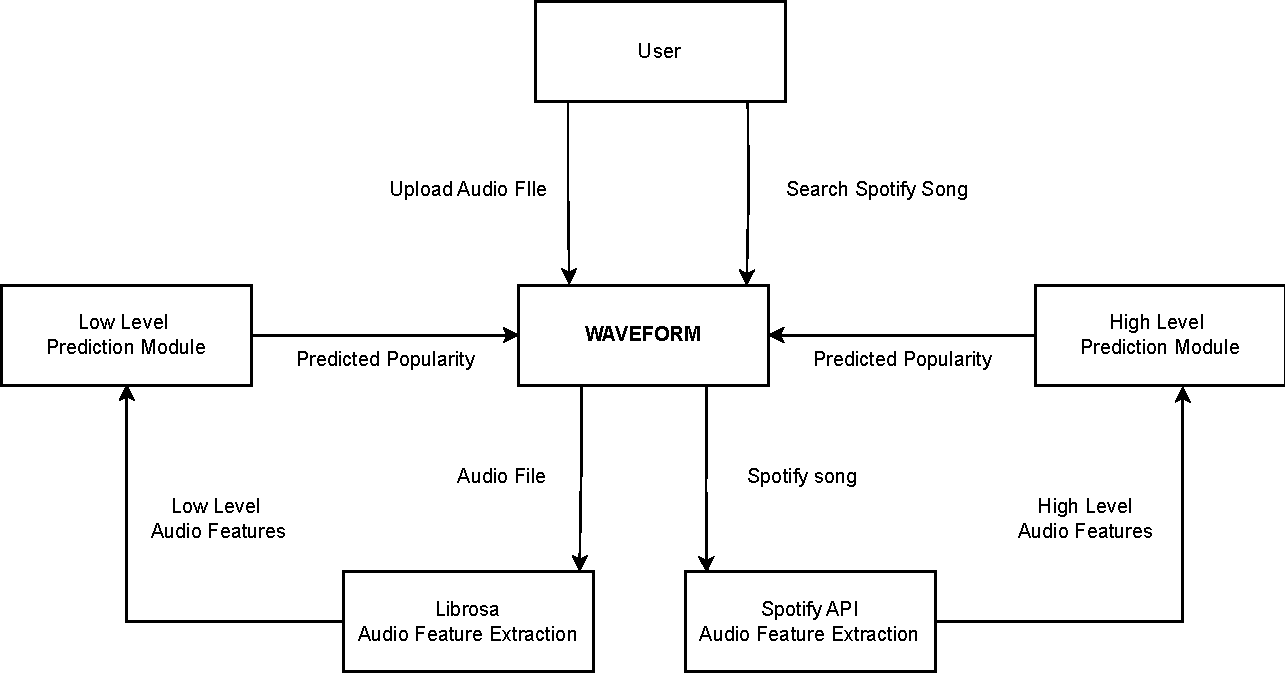
\includegraphics[scale=.8]{PDF/Sys arch.pdf}
    \caption{System Architecture}
    \label{fig:System Architecture for  Waveform}
\end{figure}

\clearpage
% \section{Input Design}
\clearpage

\section{Use Case Design}
A use case diagram is a visual representation of the interactions between user and the system. It shows the functions of the system and the actor involved in those functions in the system.It serves as a blueprint for understanding the functional requirements of a system from a user’s perspective, aiding in the communication between stakeholders and guiding the development process.

\begin{figure}[H]
    \centering
    % \includegraphics[width=13cm,height=15cm]{images/UseCase.EDITED.png}
    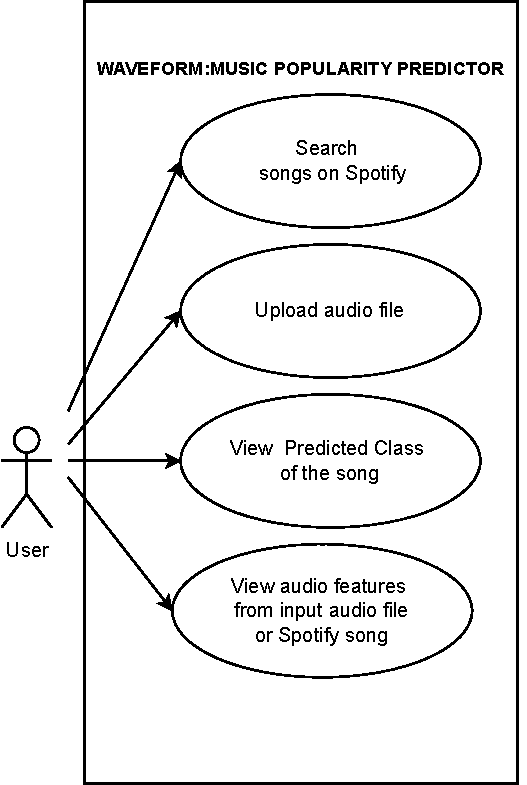
\includegraphics[scale=1]{PDF/UseCase Diagram.pdf}
    \caption{Use case Diagram}
    \label{fig:Use case diagram for Waveform}
\end{figure}
\clearpage

\section{Activity Design}
Activity diagrams are graphical representations of workflows of step-wise activities and actions with support for choice, iteration and concurrency.They are intended to model both computational and organizational processes. Activity diagrams show the overall flow of control through the system.

\begin{figure}[H]
    \centering
    % \includesvg[width=11cm,height=16cm]{SVG/Activity-main-realSVG.svg}
    % \includegraphics[width=11cm,height=16cm]{images/Activity diagram2.png}
    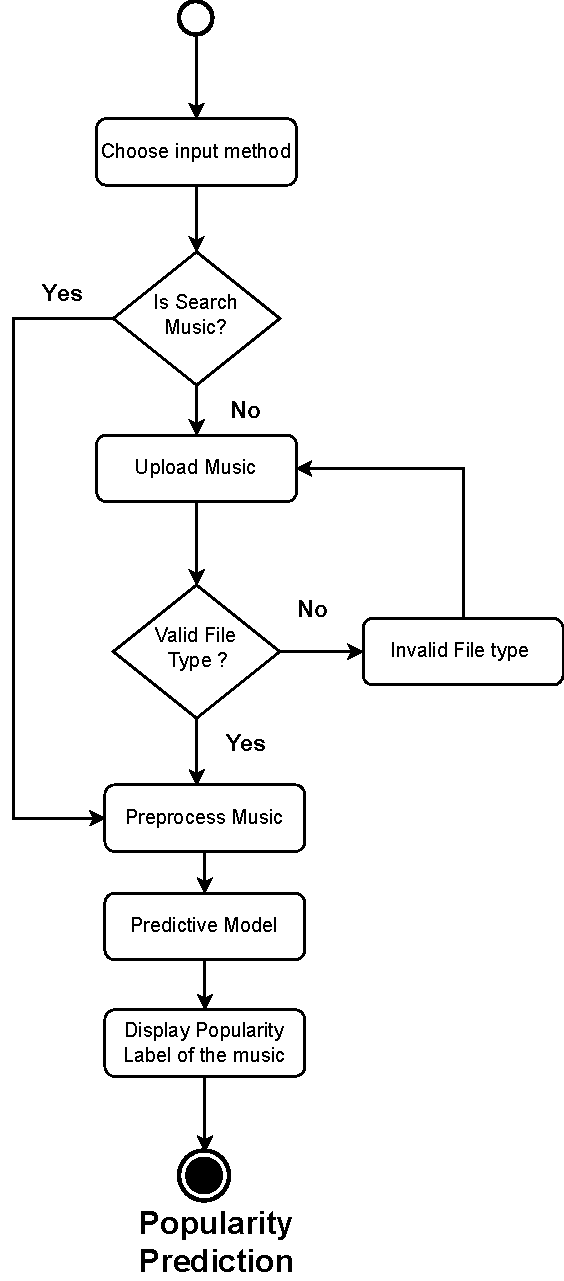
\includegraphics[scale=0.8]{PDF/Activity-main-real.pdf}
    \caption{Activity Diagram}
    \label{fig:activity diagram for Waveform}
\end{figure}


\clearpage

% \section{Database Design}

\section{Libraries and Packages Used}
\begin{itemize}
\item \textbf{Django:} A high-level Python web framework that enables rapid development of web applications, providing features such as URL routing, template engine, and ORM for database interaction.

\item \textbf{djangorestframework:} An extension for Django that facilitates building RESTful APIs, offering serialization, authentication, and request/response handling functionalities.

\item \textbf{django-rest-framework-social-oauth2:} Adds social media platform authentication capabilities to Django REST framework, allowing users to log in using accounts from platforms like Facebook or Google.

\item \textbf{drf-yasg:} A tool for generating real Swagger/OpenAPI 2.0 specifications from Django Rest Framework APIs, simplifying API documentation and testing.

\item \textbf{psycopg2-binary:} A PostgreSQL adapter for Python that enables interaction with PostgreSQL databases, providing efficient data access and manipulation capabilities.

\item \textbf{python-decouple:} A Python package that helps manage project settings in a clean, modular way by separating settings from source code, enhancing security and flexibility.

\item \textbf{librosa:} A Python package for music and audio analysis, offering tools for feature extraction, beat tracking, and spectrogram manipulation, essential for processing audio data in the project.

\item \textbf{scikit-learn:} A comprehensive machine learning library for Python, providing tools for data preprocessing, modeling, and evaluation, including algorithms for classification, regression, clustering, and dimensionality reduction.

\item \textbf{joblib:} A lightweight pipelining library for Python, primarily used for efficient caching and persistence of objects, particularly beneficial for model persistence in machine learning workflows.

\item \textbf{Pandas:} Python library for data manipulation and analysis, offering powerful tools for working with structured data efficiently.
\item \textbf{ReactJS:} For creating UI and passing data to backend.
\end{itemize}
\newpage
\section{Module Description}
\subsection*{Frontend Module:}
It is responsible for creating the user interface of the Waveform web application. It encompasses all the visual elements and interactions users encounter when using the app. This includes designing and implementing various pages such as the landing page, sign-up page, home page, predict page, results page, about page, and contact page. Components like buttons, input fields, navigation bars, and cards are constructed and styled to ensure a seamless and intuitive user experience. Additionally, the frontend module integrates with other modules like authentication, profile, high-level prediction, low-level prediction, and visualization to provide users with the functionality they need to interact with the application effectively.

\subsection*{Authentication \& Profile Module:}
The authentication and profile module handles user authentication and manages user profiles within the Waveform application. It allows users to sign up for an account using their Google credentials or log in if they already have an account. New users can provide additional information such as their date of birth and gender during the sign-up process. This module ensures that user data is securely stored and manages the association between users and their profiles. It also provides functionality for users to update their profile information and manage their account settings.

\subsection*{High Level Prediction Module:}
The high-level prediction module is responsible for predicting the overall popularity of songs based on aggregated data from the Spotify API. Users can search for songs using an autocomplete search box, and upon selecting a song, the module predicts its popularity category (hit, popular, not hit, or flop). This module utilizes machine learning models trained on Spotify audio features and artist popularity data to make accurate predictions. After prediction, users can view the predicted popularity of the selected song and explore similar songs for further analysis.

\subsection*{Low Level Prediction Module:}
The low-level prediction module enables users to upload their own audio files and predicts the popularity of those songs. Users can select an audio file, input additional information such as the track name, explicitness value, and track cover art, and submit it for processing. The module extracts various audio features from the uploaded file and utilizes a machine learning model to predict its popularity category. Users can then view the prediction results on the results page, where they can filter songs based on their prediction status (completed, in-progress, failed) and view associated details such as track name, cover art, and predicted popularity.

\subsection*{Visualization Module:}
The visualization module, also known as the Stat page, provides users with visual representations of predicted song popularity and audio features. For high-level predictions, users can view a graph illustrating the distribution of audio features, aiding in understanding the song's characteristics and predicted popularity category. For low-level predictions, users see the predicted popularity category and key audio features displayed in card format, offering a concise summary of the song's attributes and facilitating quick assessment of its potential success. This module helps users understand both the audio properties and predicted popularity of the songs they upload or search for.

\chapter{Data Flow Diagram}
The data flow diagram is a graphical representation of the flow of data through an information system, modelling its process aspects. Often they are a preliminary step used to create an overview of the System, which can later be evaluated. Data Flow Diagrams can also be used for the visualization of data processing.

\section{Level 0 DFD}
\begin{figure}[h]
    \centering
    % \includegraphics[width=0.8\linewidth]{images/DFD0-New.drawio.png}
     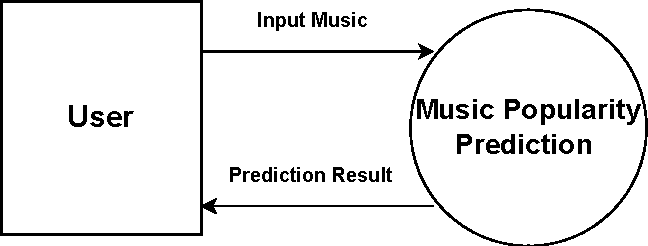
\includegraphics[scale=1]{PDF/DFD0.pdf}
    \caption{Level 0 Data Flow Diagram}
\end{figure}

\clearpage
\section{Level 1 DFD}
\\
\\

\begin{figure}[h]
    \centering
    % \includegraphics[width=1\linewidth]{images/DFD1.drawio (2).png}
    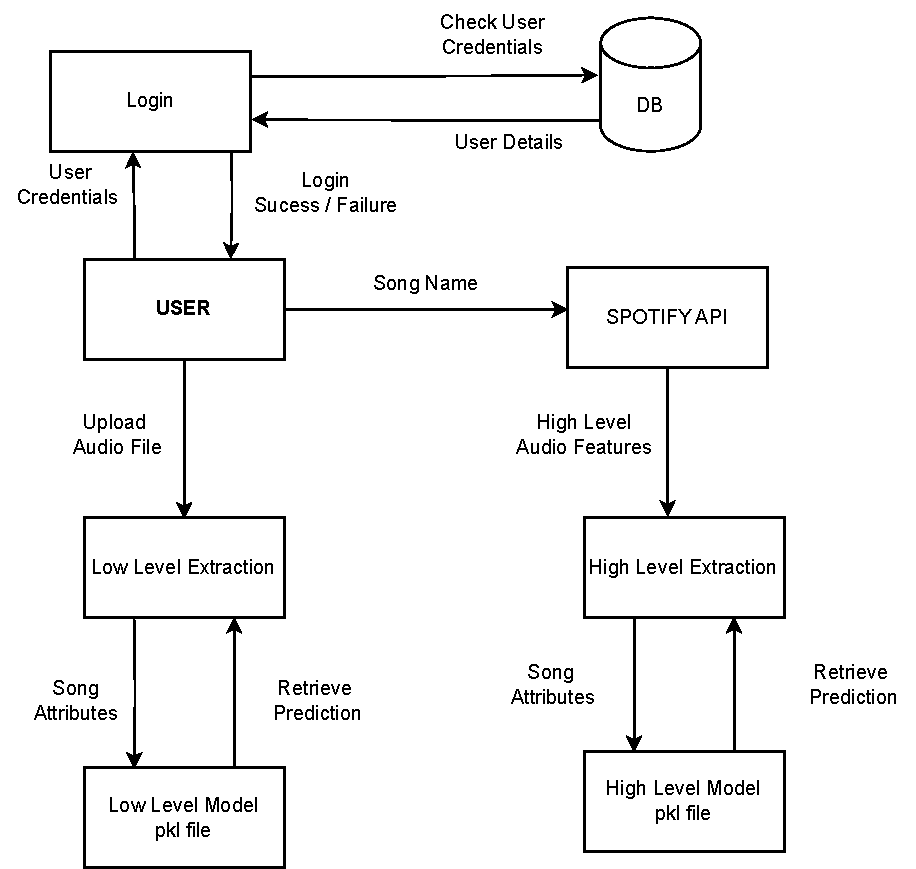
\includegraphics[width=0.8\linewidth]{PDF/DFD1.pdf}
    \caption{Level 1 Data Flow Diagram}
\end{figure}
% \section{Level 2 DFD}

\chapter{Implementation}
\section{Methodology}


\subsection{Data Collection and Preparation}

% The data preparation process involved distinct methodologies for the high-level and low-level prediction modules, each tailored to extract relevant audio features and supplementary metadata. For the high-level prediction module, we initiated the process by acquiring artist IDs from a Kaggle dataset, a repository rich in music-related data. Leveraging these IDs, we made API calls to retrieve similar artists, expanding the dataset's diversity. Next, we obtained albums and track IDs, facilitating subsequent queries to the Spotify API for extracting high-level audio features. These features encompassed various attributes such as danceability, energy, and acousticness. Additionally, to augment our dataset's richness, we aggregated the top 100 songs of each track's most popular artist, providing a broader representation of feature patterns.
% \\ \\
% On the other hand, the low-level prediction module necessitated a distinct approach. Here, we resorted to web scraping techniques to gather audio previews, which were subsequently processed using the librosa library to extract low-level audio features. However, this process was resource-intensive, demanding substantial time and storage due to the sheer volume of audio data involved. In tandem with audio feature extraction, we integrated supplementary metadata sourced from the Spotify API, including release year and track popularity
% \\ \\
% After acquiring the data, we performed preprocessing steps to prepare it for modeling. This included handling missing values, encoding categorical variables, and addressing class imbalance. Categorical variables were encoded using techniques such as one-hot encoding to convert them into numerical representations suitable for machine learning algorithms. To address class imbalance, we applied the Synthetic Minority Over-sampling Technique (SMOTE) to the training data. This technique generates synthetic samples for the minority class, ensuring a balanced distribution of classes for more robust model training. By oversampling the minority class, SMOTE helps the model learn from all available data points, improving its ability to generalize better to unseen data. 
% \\ \\ 
% During the exploratory data analysis phase, we utilized various visualization techniques such as histograms, scatter plots, and box plots to understand the distribution of features and their relationships with the target variable. Histograms provided insights into the distribution of numerical features, while scatter plots allowed us to explore relationships between pairs of variables. Box plots were particularly helpful in identifying potential outliers in the data. Additionally, we performed correlation analysis to identify features strongly associated with the target variable, guiding our feature selection process and informing our modeling approach.

The data preparation involved two main steps for high-level and low-level prediction modules. For the high-level module, we acquired artist IDs from a Kaggle dataset and expanded diversity by retrieving similar artists through API calls. We extracted high-level audio features from the Spotify API, such as danceability and energy, and augmented the dataset by aggregating top songs of each track's most popular artist. The low-level module involved web scraping audio previews and extracting low-level audio features using the librosa library. Supplementary metadata from Spotify API, including release year and track popularity, was integrated. Preprocessing steps included handling missing values, encoding categorical variables, and addressing class imbalance using SMOTE. Exploratory data analysis used histograms, scatter plots, and box plots to understand feature distributions and relationships with the target variable. Correlation analysis guided feature selection and modeling.


\subsection{{Model Training and Selection}}

% In the model training and selection phase for both the high-level and low-level prediction modules, we applied various machine learning algorithms to train our models and select the best performing ones. After preprocessing the data, which included handling missing values, encoding categorical variables, and scaling features, we split the dataset into training and testing sets. This step ensured that our models were trained on a portion of the data and evaluated on a separate portion to assess their generalization performance accurately. 
% \\ \\ 
% For the high-level prediction module, we trained several models, including Random Forest, AdaBoost, and XGBoost classifiers. These models were trained using cross-validation techniques to find the best hyperparameters. Cross-validation helped us assess the model's performance more robustly by splitting the training data into multiple subsets and training the model on each subset while evaluating it on the remaining data. Our experimentation revealed that the XGBoost classifier consistently outperformed other models in predicting song popularity.
% \\ \\
% Similarly, for the low-level prediction module, we followed a similar approach. After preprocessing the data, which included feature scaling and encoding categorical variables, we trained several models, including Random Forest, AdaBoost, and XGBoost classifiers. These models were also trained using cross-validation techniques to find the best hyperparameters.
% Our experimentation again revealed that the XGBoost classifier yielded the highest performance in predicting song popularity using low-level audio features.
% \\ \\
% Throughout the training and selection process, we carefully evaluated each model's performance using various metrics such as accuracy, precision, recall, and F1-score. Additionally, we analyzed the confusion matrix to understand the model's strengths and weaknesses better. This iterative process allowed us to identify the most suitable algorithm for each prediction module, with the XGBoost classifier being the preferred choice for both high-level and low-level prediction tasks.

In the model training and selection phase for both high-level and low-level prediction modules, we applied various machine learning algorithms and split the data into training and testing sets after preprocessing. For the high-level module, we trained Random Forest, AdaBoost, and XGBoost classifiers using cross-validation to find the best hyperparameters. XGBoost consistently outperformed other models in predicting song popularity. Similarly, for the low-level module, we followed a similar approach and found that XGBoost yielded the highest performance. We evaluated each model's performance using metrics like accuracy, precision, recall, and F1-score, along with analyzing the confusion matrix. This iterative process led us to choose the XGBoost classifier as the preferred algorithm for both prediction tasks.


\subsection{{Model Evaluation and Analysis}}
% In the model evaluation and analysis phase for both the high-level and low-level prediction modules, we embarked on a comprehensive assessment of our trained models to gauge their performance in predicting song popularity. Using a variety of evaluation metrics such as accuracy, precision, recall, and F1-score, we meticulously scrutinized the efficacy of each model in capturing the nuances of music popularity. We began by examining the accuracy of our models, which measures the proportion of correctly predicted instances. While accuracy provides an overall view of model performance, we also explored precision and recall. Precision reflects the proportion of true positive predictions among all positive predictions, indicating the model's ability to avoid false positives. Recall, on the other hand, measures the proportion of true positive predictions identified correctly, offering insights into the model's ability to capture all positive instances. Additionally, we employed the F1-score, which is the harmonic mean of precision and recall, providing a balanced assessment of model performance. 
% \\ \\ 
% By considering both precision and recall, the F1-score offers a more holistic evaluation, particularly useful when dealing with imbalanced datasets, such as those in popularity prediction. Furthermore, we delved into the confusion matrix, a tabular representation that summarizes the model's performance by comparing predicted labels with actual labels. Analyzing the confusion matrix allowed us to identify patterns of correct and incorrect predictions, aiding in understanding the strengths and weaknesses of our models.
% \\ \\
% To optimize the performance of our models further, we leveraged advanced optimization techniques such as grid search and randomized search to fine-tune the hyperparameters of the XGBoost classifier. These techniques systematically explored different parameter combinations, aiming to identify the optimal configuration that maximized prediction accuracy. Our analysis revealed that the XGBoost model consistently outperformed other algorithms in both the high-level and low-level prediction modules for song popularity. Its robustness and adaptability proved invaluable in accurately predicting song popularity and extracting low-level audio features. This reaffirmed the XGBoost model's effectiveness as a powerful tool in our music popularity prediction system, providing users with reliable and insightful predictions for informed decision-making.

In the model evaluation phase, we assessed our trained models' performance in predicting song popularity using various metrics like accuracy, precision, recall, and F1-score. We examined precision and recall to gauge the models' ability to avoid false positives and capture all positive instances, respectively. The F1-score provided a balanced assessment considering both metrics. We analyzed the confusion matrix to identify patterns of correct and incorrect predictions, helping understand our models' strengths and weaknesses. To optimize our models further, we used techniques like grid search and randomized search to fine-tune the XGBoost classifier's hyperparameters. Our analysis showed that the XGBoost model consistently outperformed others in both high-level and low-level prediction modules, confirming its effectiveness in accurately predicting song popularity and extracting low-level audio features.
This confirmed XGBoost's effectiveness in our music popularity prediction system, providing reliable predictions for decision-making.

\section{Algorithms}

\subsection{Random Forest Classifier:}
  In our project, the Random Forest Classifier was utilized to predict the popularity of songs based on their audio features. Random Forest is an ensemble learning method that constructs a multitude of decision trees during training and outputs the mode of the classes (classification) or the mean prediction (regression) of the individual trees. It is known for its robustness and ability to handle complex datasets with high dimensionality. For our task, Random Forest proved to be effective in capturing the non-linear relationships between audio features and song popularity. Additionally, Random Forest provides feature importances, allowing us to identify which audio features contribute most significantly to the prediction of song popularity, aiding in feature selection and model interpretation.


\subsection{AdaBoost Classifier:}
   We also employed the AdaBoost Classifier to predict song popularity. AdaBoost, short for Adaptive Boosting, is another ensemble learning method that combines multiple weak learners to create a strong classifier. It focuses on improving the accuracy of weak classifiers by assigning higher weights to misclassified data points. In our project, AdaBoost was effective in boosting the performance of models and reducing overfitting, leading to more accurate predictions of song popularity. AdaBoost's iterative nature and ability to adapt to misclassified instances make it well-suited for handling complex datasets with noise and outliers. Moreover, AdaBoost's simplicity and versatility make it suitable for integration with other classifiers in ensemble methods, enhancing prediction accuracy further.


\subsection{XGBoost Classifier:}
   XGBoost, an implementation of gradient boosting machines, played a crucial role in our project for predicting song popularity. It uses a technique called gradient boosting to iteratively add new models to correct the errors made by existing models. XGBoost is widely known for its speed, performance, and ability to handle large datasets. In our project, XGBoost demonstrated excellent predictive power and versatility, making it a valuable addition to our ensemble of classifiers. XGBoost's advanced regularization techniques, including L1 and L2 regularization, help prevent overfitting and improve generalization performance. Furthermore, XGBoost's support for parallel and distributed computing allows for efficient training on large-scale datasets, making it suitable for real-world applications with extensive data volumes.

\section{Development Tools}

\subsection*{Backend}
For backend development, we utilized Django REST Framework (DRF), a powerful toolkit for building Web APIs in Python. DRF provided us with a range of features for creating RESTful APIs, including serialization, authentication, and class-based views. It allowed us to quickly develop scalable and maintainable APIs to interact with our frontend applications or external clients.
\subsection*{Frontend}
On the frontend, we built our web application using React, a popular JavaScript library for building user interfaces. React's component-based architecture enabled us to create reusable UI components, resulting in a more modular and organized codebase. This approach facilitated efficient development and maintenance of the user interface, allowing us to deliver a responsive and intuitive application to our users.
\subsection*{Machine Learning Tools}
\begin{itemize}
    \item \textbf{scikit-learn:}
    \begin{enumerate}
        \item \textbf{fit:} This function is used to train a machine learning model on the training data.
        \item \textbf{predict:} After training, this function is used to make predictions on new data.
        \item \textbf{accuracy\_score:} This function calculates the accuracy of the model's predictions compared to the true labels.
    \end{enumerate}
\end{itemize}

\begin{itemize}
    \item \textbf{librosa:}
    \begin{enumerate}
        \item \textbf{load:} This function is used to load audio files and return the audio data and sampling rate.
        \item \textbf{amplitude\_to\_db:} This function is used to convert amplitude to decibels.
        \item \textbf{beat.beat\_track:} It estimates the tempo (beats per minute) of a signal.
    \end{enumerate}
\end{itemize}

\begin{itemize}
    \item \textbf{Matplotlib:}
    \begin{enumerate}
        \item \textbf{plot:} This function is used to create various types of plots, including line plots, scatter plots, and histograms.
        \item \textbf{xlabel and ylabel:} These functions are used to label the x and y axes of plots, respectively.
        \item \textbf{boxplot:} This function is used to create boxplots to visualize the distribution of data.
    \end{enumerate}
\end{itemize}

\begin{itemize}
    \item \textbf{joblib:}
    \begin{enumerate}
        \item \textbf{dump:} This function is used to save the trained model to a file.
        \item \textbf{load:} This function is used to load a trained model from a file.
    \end{enumerate}
\end{itemize}

\begin{itemize}
    \item \textbf{Pandas:}
    \begin{enumerate}
        \item \textbf{read\_csv:} This function is used to read data from a CSV file into a DataFrame.
        \item \textbf{merge:} This function is used to merge DataFrame objects by performing a database-style join operation.
        \item \textbf{drop\_duplicates:} This function is used to remove duplicate rows from a DataFrame.
    \end{enumerate}
\end{itemize}




\chapter{Testing}
 Software testing involves the execution of a software component or system component to evaluate one or more properties of interest. In general, these properties indicate the extent to which the component or system under test:
\begin{itemize}
    \item Meets the requirements that guided its design and development.
    \item Responds correctly to all kinds of song input.
    \item Performs its functions within a short time.
\end{itemize}

\section{Testing Methodologies}
Software testing methodologies are for making sure that the software products/systems developed have been successfully tested to meet their specified requirements and can successfully operate.\\

\section{Unit Testing}
 Unit testing is a software development process in which the smallest testable parts of an application, called units, are individually and independently scrutinized for proper operation.
\subsection{Frontend Module}
The frontend module is responsible for creating the user interface of the Waveform web application.

\subsubsection*{UI Interaction}
\textbf{Steps:}
\begin{itemize}
    \item Run the application and interact with the UI.
\end{itemize}
\textbf{Expected Output:}
\begin{itemize}
    \item Ensure search fields and name boxes are all active and user is able to input values into the various fields.
    \item Navigation buttons and links are properly placed and are clickable to the user.
    \item  UI cards that adjust according to the viewport size of the page.
    \item Clickable buttons that calls the functions for execution
\end{itemize}
\textbf{Status:}
\begin{itemize}
    \item Pass
\end{itemize}

\subsection{Authentication \& Profile Module}
The authentication and profile module handles user authentication and manages user profiles within the Waveform application.

\subsubsection*{User Authentication}
\textbf{Steps:}
\begin{itemize}
    \item Sign up for a new account using Google credentials.
    \item Log in with the newly created account.
\end{itemize}
\textbf{Expected Output:}
\begin{itemize}
    \item Ensure successful account creation and login process.
\end{itemize}
\textbf{Status:}
\begin{itemize}
    \item Pass
\end{itemize}

\subsection{High Level Prediction Module}
The high-level prediction module predicts the o popularity of songs already present in Spotify based on aggregated data from the Spotify API.

\subsubsection*{Song Prediction}
\textbf{Steps:}
\begin{itemize}
    \item Search for a song using the autocomplete search box.
    \item Select a song from the search results.
    \item Redirect to Song information page and view song details \& similar songs
    \item Click predict button to view song popularity and song attributes
\end{itemize}
\textbf{Expected Output:}
\begin{itemize}
    \item Ensure accurate prediction of the song's popularity category (hit, popular, not hit, or flop).
\end{itemize}
\textbf{Status:}
\begin{itemize}
    \item Pass
\end{itemize}

\subsection{Low Level Prediction Module}
The low-level prediction module enables users to upload their own audio files and predicts the popularity of those songs with the help of Librosa package.

\subsubsection*{Audio File Upload}
\textbf{Steps:}
\begin{itemize}
    \item Select an audio file for upload from the deivce.
    \item Input additional information such as track name and explicitness value.Optionally,user can choose to input a image for the song ,else default image will be kept with the song
    \item Submit the file for processing.
\end{itemize}
\textbf{Expected Output:}
\begin{itemize}
    \item Ensure successful upload.
    \item Song status is updated in Results page.
    \item When prediction is complete , song status is changed to completed.
    \item Prediction of the uploaded audio file along with song attribute values used for prediction, can be viewed in stats page.
\end{itemize}
\textbf{Status:}
\begin{itemize}
    \item Pass
\end{itemize}

\subsection{Visualization Module}
The visualization module provides users with visual representations of predicted song popularity and audio features.

\subsubsection*{Data Visualization}
\textbf{Steps:}
\begin{itemize}
    \item View a graph illustrating the distribution of audio features for a selected song.
\end{itemize}
\textbf{Expected Output:}
\begin{itemize}
    \item Ensure clear and accurate representation of audio feature distribution.
\end{itemize}
\textbf{Status:}
\begin{itemize}
    \item Pass
\end{itemize}


 \section{Integration Testing}
  Integration testing is the phase is software testing in which individual software modules are combined and tested as a group.
 \begin{itemize}
   \item \textbf{UI Integration:}
    \begin{itemize}
        \item Description: Test whether users can interact with the Waveform's user interface elements effectively, including input methods such as the search input box, signup form, and song upload form, as well as displaying uploaded songs and their attributes.
        \item Status: Pass
    \end{itemize}
\item \textbf{Authentication \& Profile Integration:}
    \begin{itemize}
        \item Description: Verify that users can be  authenticated and  given access their unique profiles within the Waveform application using Google Authentication for both account creation and login. Ensure that users can view personal uploads and their associated results.
        \item Status: Pass
    \end{itemize}
       
     \item \textbf{Upload \& Search Integration: }\\
     This integration allows users to search songs on spotify and upload songs from their device in a single page.
     \begin{itemize}
    \item Description: Testing on the Spotify song autocomplete feature and duration of user-uploaded song.
    \item Status: Pass
    \end{itemize}
     
      \item \textbf{Low End Module Integration:}
    \begin{itemize}
        \item Description: Test the integration of low-end module, Verify that upon successful upload, the song's status is updated within the application, reflecting its processing stage. Ensure users can monitor progress, and once prediction is complete, the song status transitions to "completed," with predicted class and song attribute values visible in the statistics page.
        \item Status: Pass
    \end{itemize}

    \item \textbf{High End Module Integration:}
    \begin{itemize}
        \item Description: Validate the integration of high-end module, utilizing aggregated data from the Spotify API to predict the popularity of songs available on Spotify. Test whether users can search for songs, select a song from the results, and view its details and similar songs. Verify that by clicking the predict button, users receive insights into the song's predicted popularity category, ranging from "hit" to "flop." Ensure that this prediction is based on comprehensive analysis, aiding users in making informed decisions regarding song selection or exploration.
        \item Status: Pass
    \end{itemize}    
 \end{itemize}
 
 
 \clearpage
 \section{System Testing}
 System testing of software or hardware is testing conducted on a complete, integrated system to evaluate the systems compliance with its specific requirements. System testing falls within the scope of black-box testing, and as such, should require no knowledge of the inner design of the code or logic.
\begin{itemize}

\item T01
    \begin{itemize}
        \item Test Case Title: Uploading a song
        \item Test Condition: Check the duration of the song upload for issues
       \item System Behavior: The system processes the uploaded song and checks for any duration-related issues
        \item Expected Result: The duration of the uploaded song is checked, and any issues related to it are identified.
        \item Actual Result: The duration of the uploaded song is checked, and no issues are found.
        \item Status: Pass
    \end{itemize}
    \item T02
    \begin{itemize}
        \item Test Case Title: Extracting audio features from a song
        \item Test Condition: Inputting a music track for feature extraction
        \item System Behavior: The system utilizes Spotify API and Librosa to extract audio features
        \item Expected Result: Audio features such as tempo, danceability, energy, and valence are extracted accurately.
        \item Actual Result: Audio features such as tempo, danceability, energy, and valence are extracted accurately.
        \item Status: Pass
    \end{itemize}
    
    \item T03
    \begin{itemize}
        \item Test Case Title: Training the Classification Model
        \item Test Condition: Providing labeled data for training the high-level classification model
        \item System Behavior: Machine learning algorithms to train the model
        \item Expected Result: Categorized songs into four popularity categories
        \item Actual Result: Categorized songs into four popularity categories
        \item Status: Pass
    \end{itemize}

    
\end{itemize}


\chapter{Graphical User Interface}
GUI stands for Graphical User Interface, which is a software program that uses visual elements to allow users to interact with a computer or website.

\section{Main GUI Components}
Pages in a web application serve as interactive visual interfaces for users to navigate and interact with content and functionality. The main GUI components present include:

\begin{itemize}
    \item Landing Page:
    \begin{itemize}[label=--]
        \item Sign in with Google button
        \item About Waveform
    \end{itemize}
    
    \item SignUp Page:
    \begin{itemize}[label=--]
        \item Date of Birth Selector
        % \item Profile Picture Upload button
        \item Create Account button
    \end{itemize}
    
    \item Navbar:
    \begin{itemize}[label=--]
        \item Home
        \item Results
        \item About
        \item Contact Us
        \item Profile button
        \item Logout button
    \end{itemize}
    
    \item Home Page:
    \begin{itemize}[label=--]
        \item Spotify Autocomplete Searchbox
        \item Song Upload Area
        \item New Releases Cards
    \end{itemize}
    
    \item Predict Page:
    \begin{itemize}[label=--]
        \item Song Track Spotify Embed
        \item Predict button
        \item Similar Song Cards
    \end{itemize}
    
    \item Stat Page:
    \begin{itemize}[label=--]
        \item Song Cover Image
        \item Text field for track name
        \item Text field to display predicted song popularity
        \item Cards to display duration, tempo, loudness, and key
        \item Graph to visualize audio features
    \end{itemize}
    
    \item Results Page:
    \begin{itemize}[label=--]
        \item Selector for Completed, Pending, Failed predictions
        \item Cards to display track and its prediction
    \end{itemize}

    \item Profile Page:
    \begin{itemize}[label=--]
        \item Upload Profile Photo
        \item Edit Name and DOB
    \end{itemize}
    
    \item About Page:
    \begin{itemize}[label=--]
        \item Description of Waveform
        \item Team Member details
    \end{itemize}
    
    \item Contact Page:
    \begin{itemize}[label=--]
        \item Form for collecting information as message to the developers
        \item Submit button
    \end{itemize}
\end{itemize}

The working of the GUI can be explained in a sequence of events as listed below:
   \begin{itemize}
    \item \textbf{Authentication Flow:}
    \begin{enumerate}
        \item Open Waveform web application.
        \item User clicks "Sign in with Google" button.
        \item If the user is new, they're redirected to the SignUp page to create an account.
        \item If the user already has an account, they're redirected to the Home page.
    \end{enumerate}
    
    \item \textbf{High Level Prediction Flow:}
    \begin{enumerate}
        \item User searches for a song name in the autocomplete searchbox.
        \item Clicks on the interested track.
        \item User is redirected to the Predict Page, where the song embed, similar songs, and predict button are visible.
        \item Clicks on the predict button.
        \item Redirects to the Stat page.
        \item User can now view the audio feature visualization and the predicted song popularity.
    \end{enumerate}
    
    \item \textbf{Low Level Prediction Flow:}
    \begin{enumerate}
        \item Clicks on the upload song button in Home page.
        \item Selects the audio file, inputs track name, and track cover art, with explictiness value (0 or 1), and clicks submit.
        \item The song file is uploaded, and processing starts.
        \item After a while, the user clicks on the Results page.
        \item Selector of Completed, Pending, Failed can be used to filter the songs.
        \item Cards of songs, have the associated audio file, track name, track cover art, and predicted popularity.
    \end{enumerate}
\end{itemize}

\newpage

\section{Screenshots}
\begin{figure}[h]
    \centering
    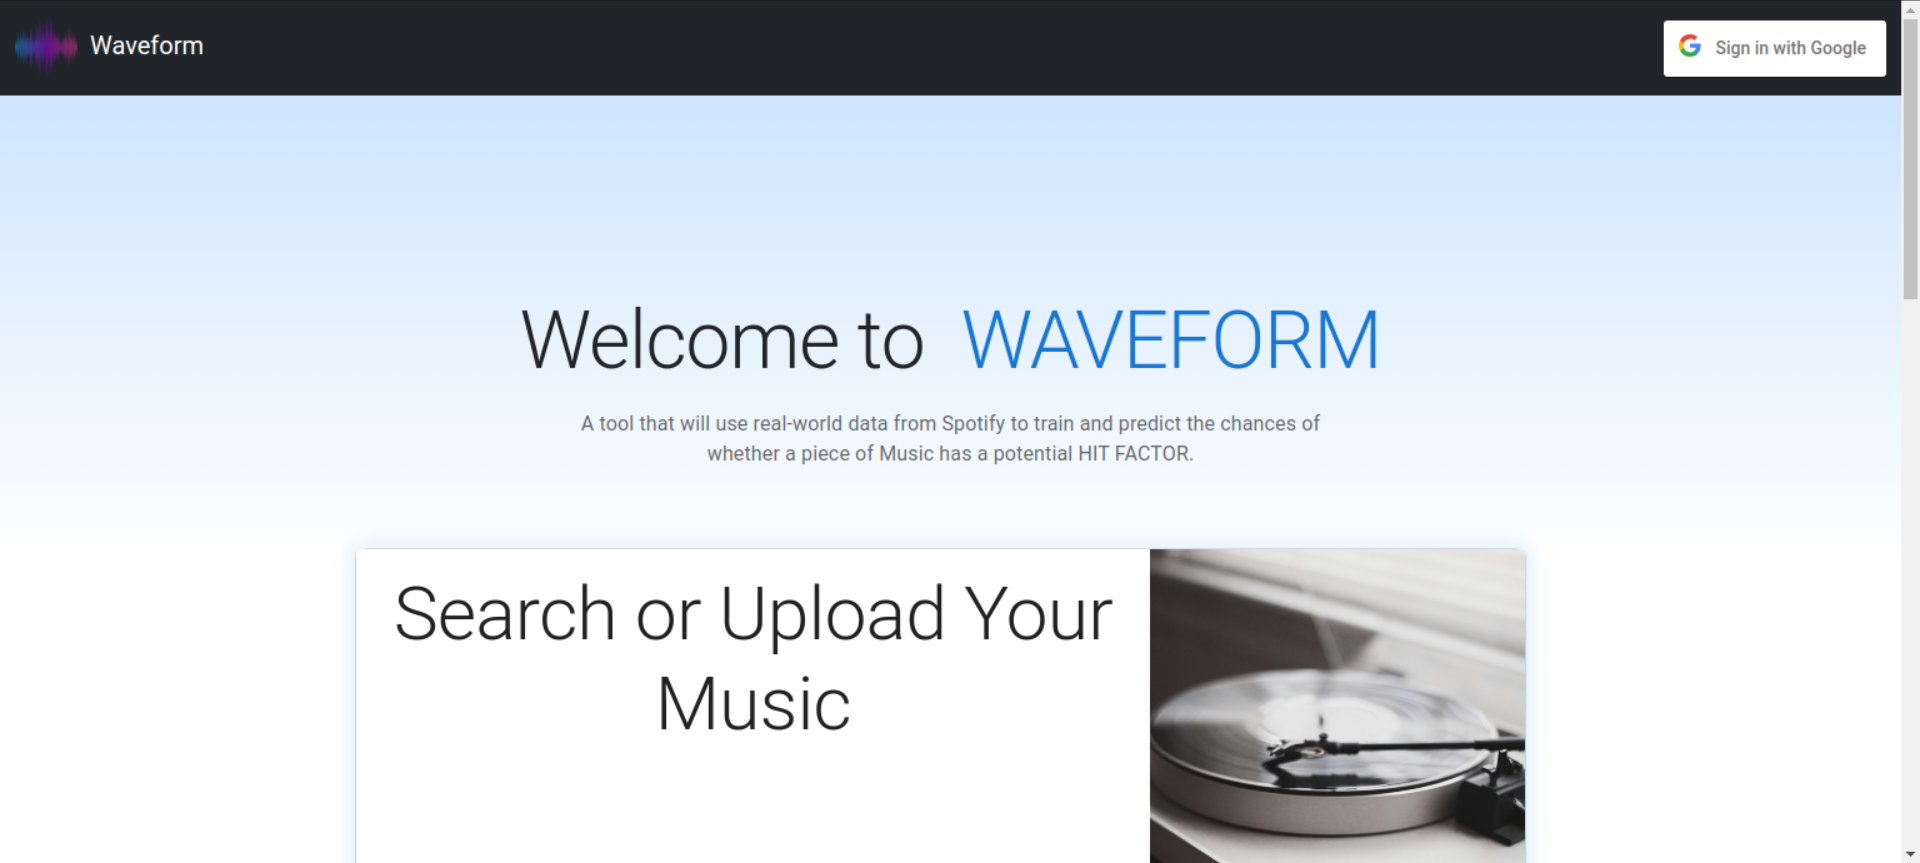
\includegraphics[width=.95\linewidth]{screenshots/1.landing.png}
    \caption{Landing page}
  
\end{figure}

\begin{figure}[h]
    \centering
    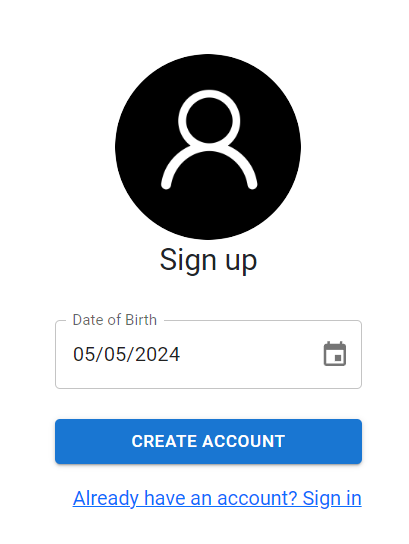
\includegraphics[width=.33\linewidth]{screenshots/2.signup.png}
    \caption{Sign Up}
    
\end{figure}
\clearpage
\begin{figure}[h]
    \centering
    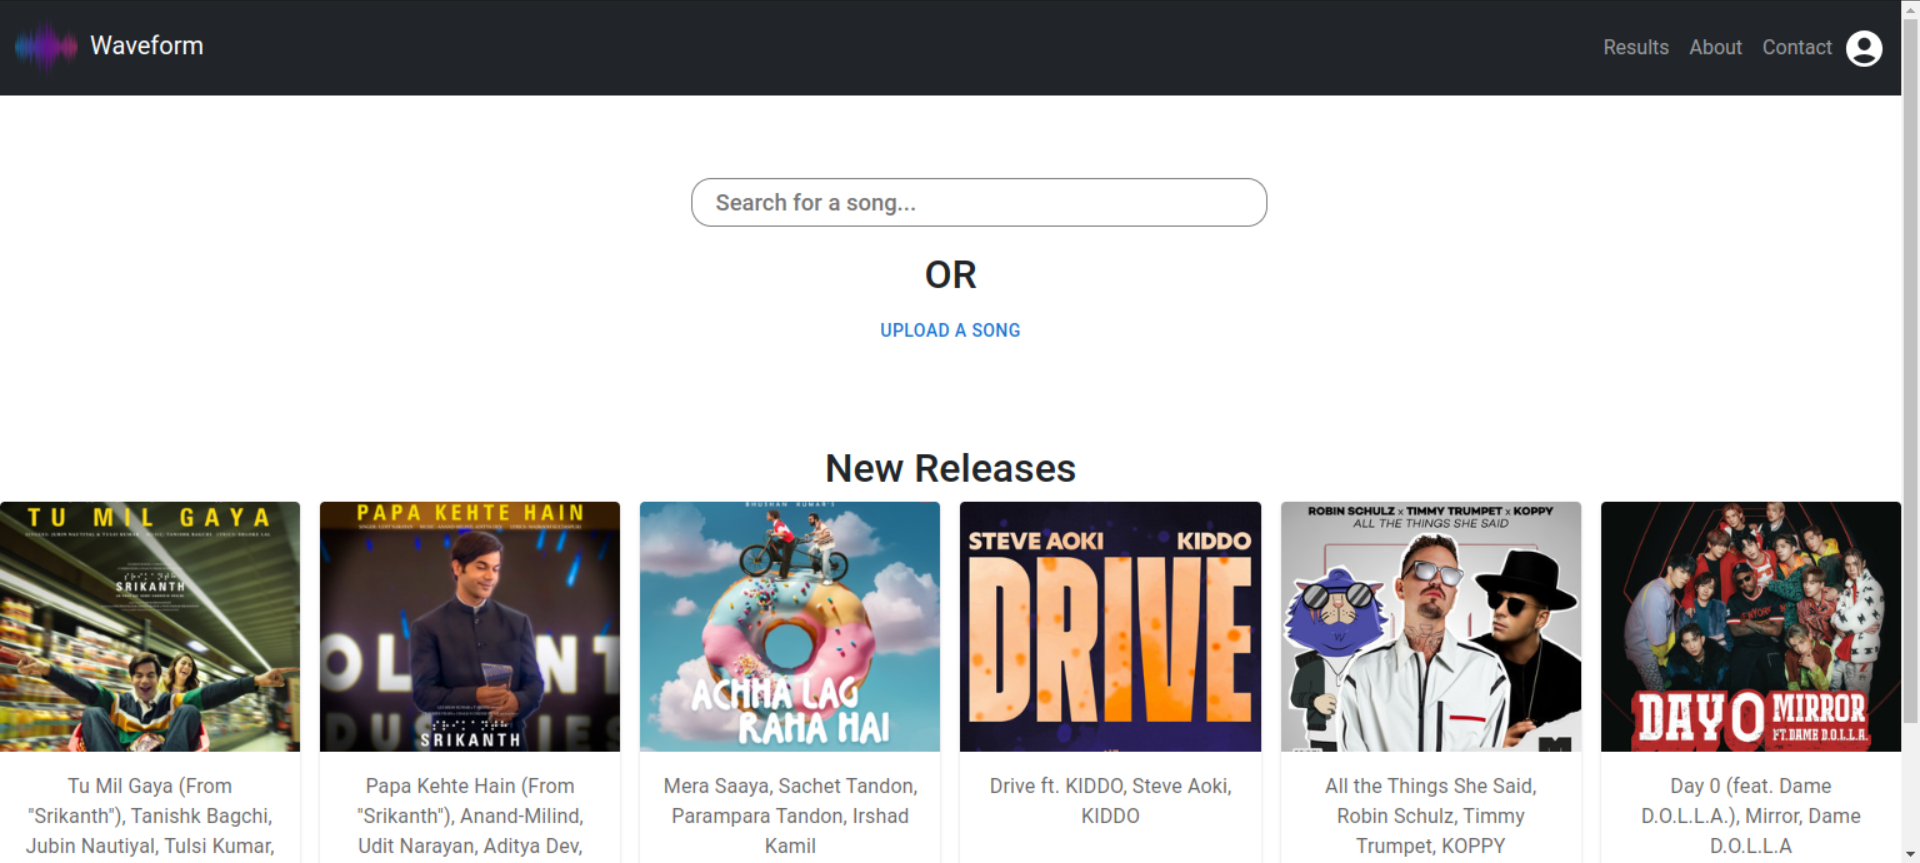
\includegraphics[width=.95\linewidth]{screenshots/3.homepage.png}
    \caption{Home Page}
    
\end{figure}

\begin{figure}[h]
    \centering
    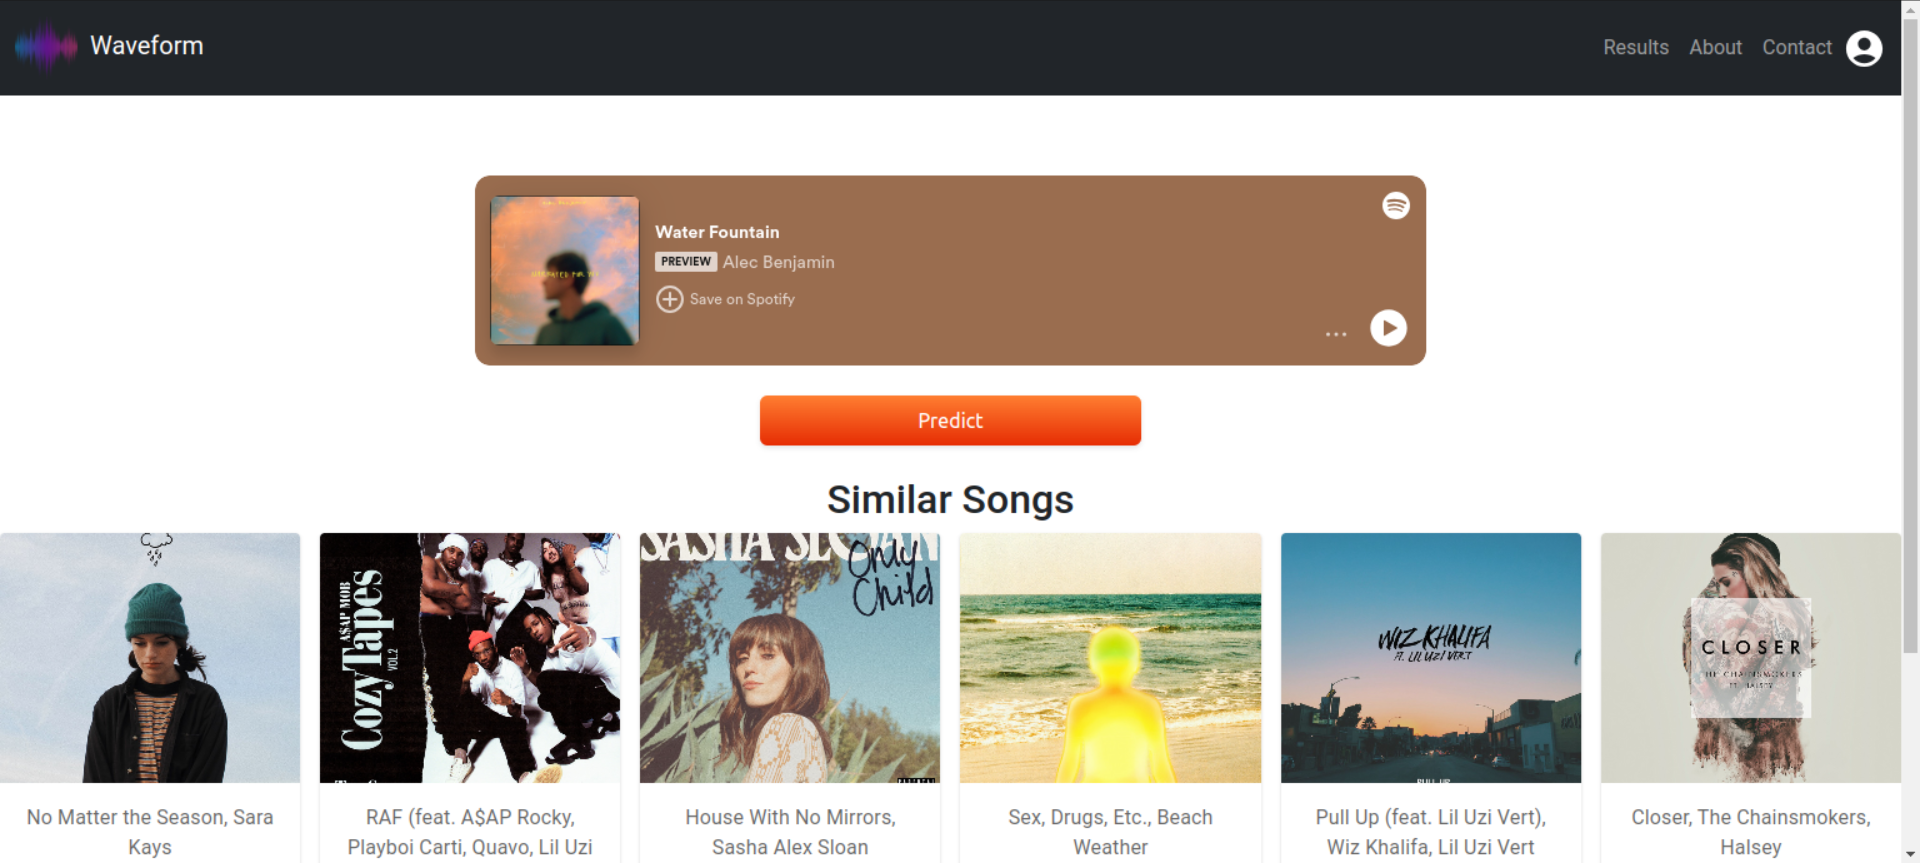
\includegraphics[width=1\linewidth]{screenshots/4.predict.png}
    \caption{Predict Page}
   
\end{figure}

\begin{figure}[h]
    \centering
    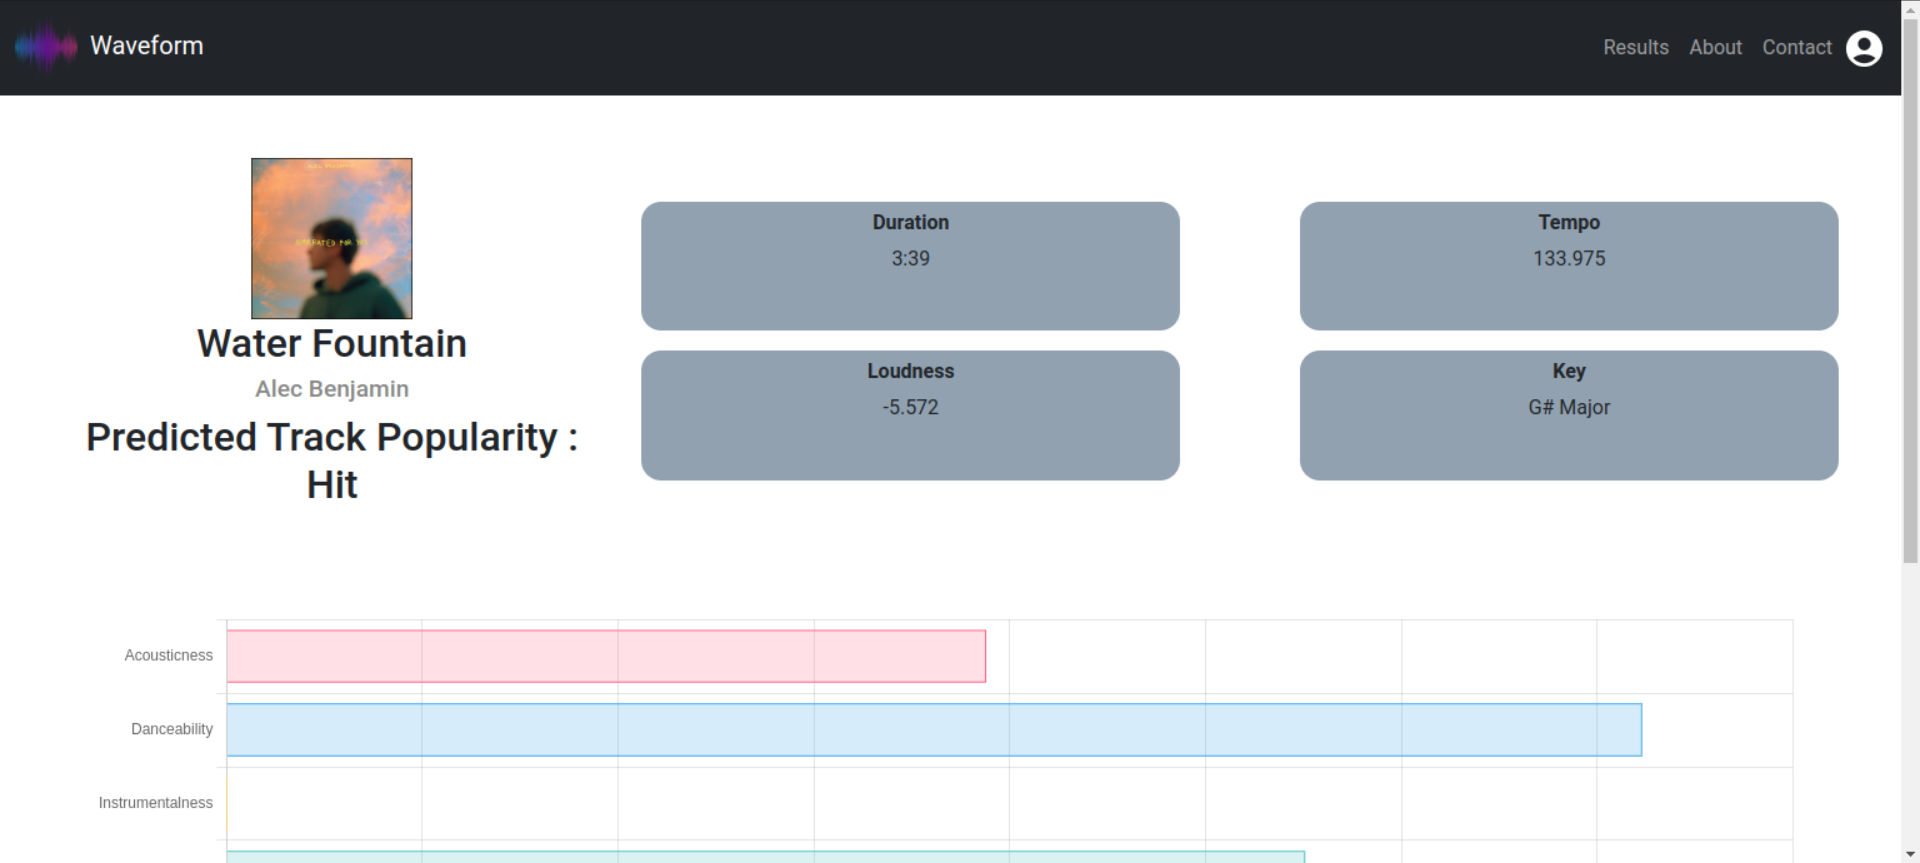
\includegraphics[width=1\linewidth]{screenshots/5.stat.png}
    \caption{Stat Page-I}
  
\end{figure}

\begin{figure}[h]
    \centering
    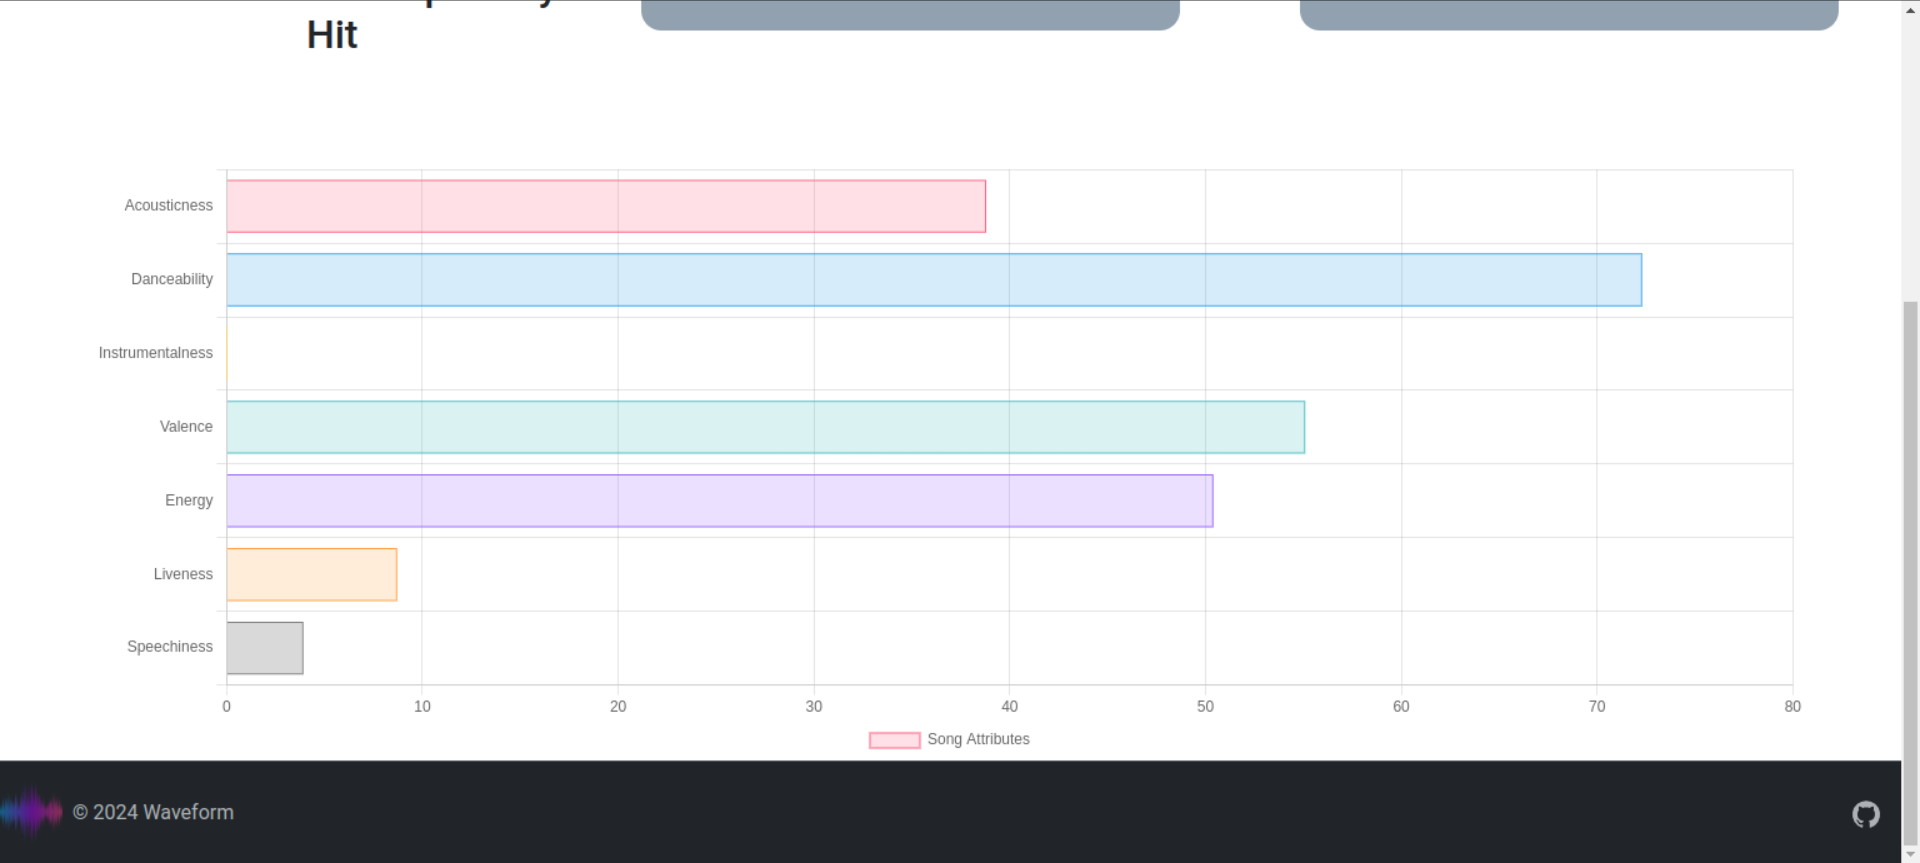
\includegraphics[width=\linewidth]{screenshots/6.stat.png}
    \caption{Stat Page-II}
   
\end{figure}

\begin{figure}[h]
    \centering
    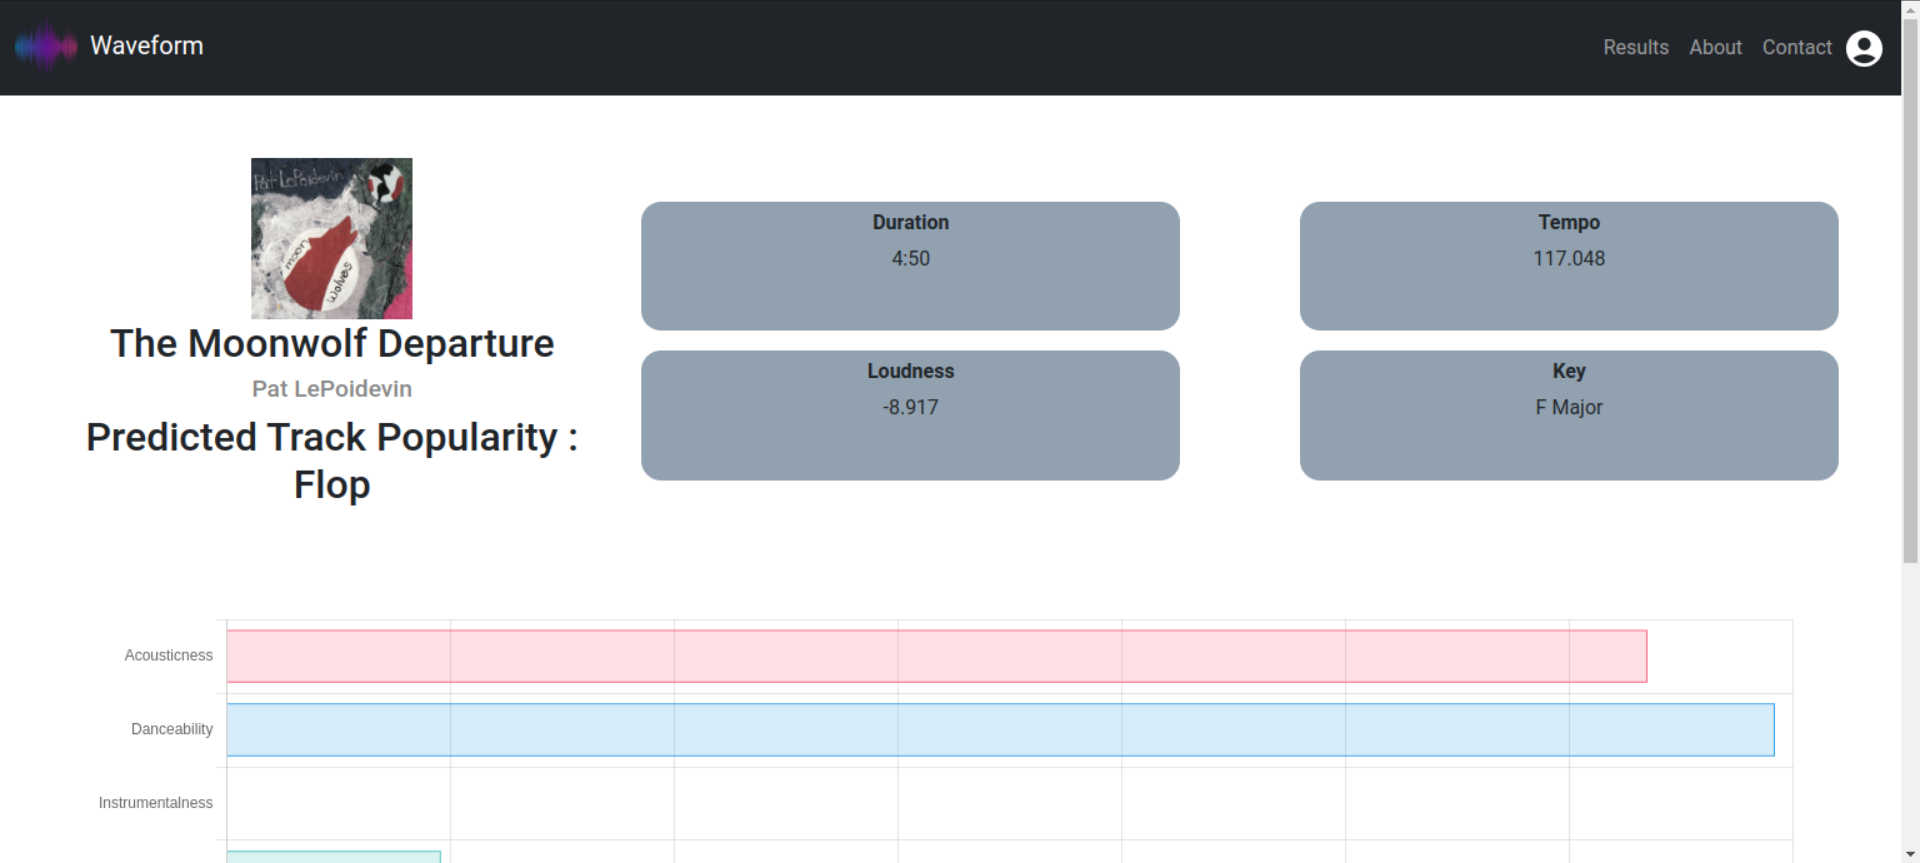
\includegraphics[width=1\linewidth]{screenshots/7.stat.png}
    \caption{Stat Page-III}

\end{figure}

\begin{figure}[h]
    \centering
    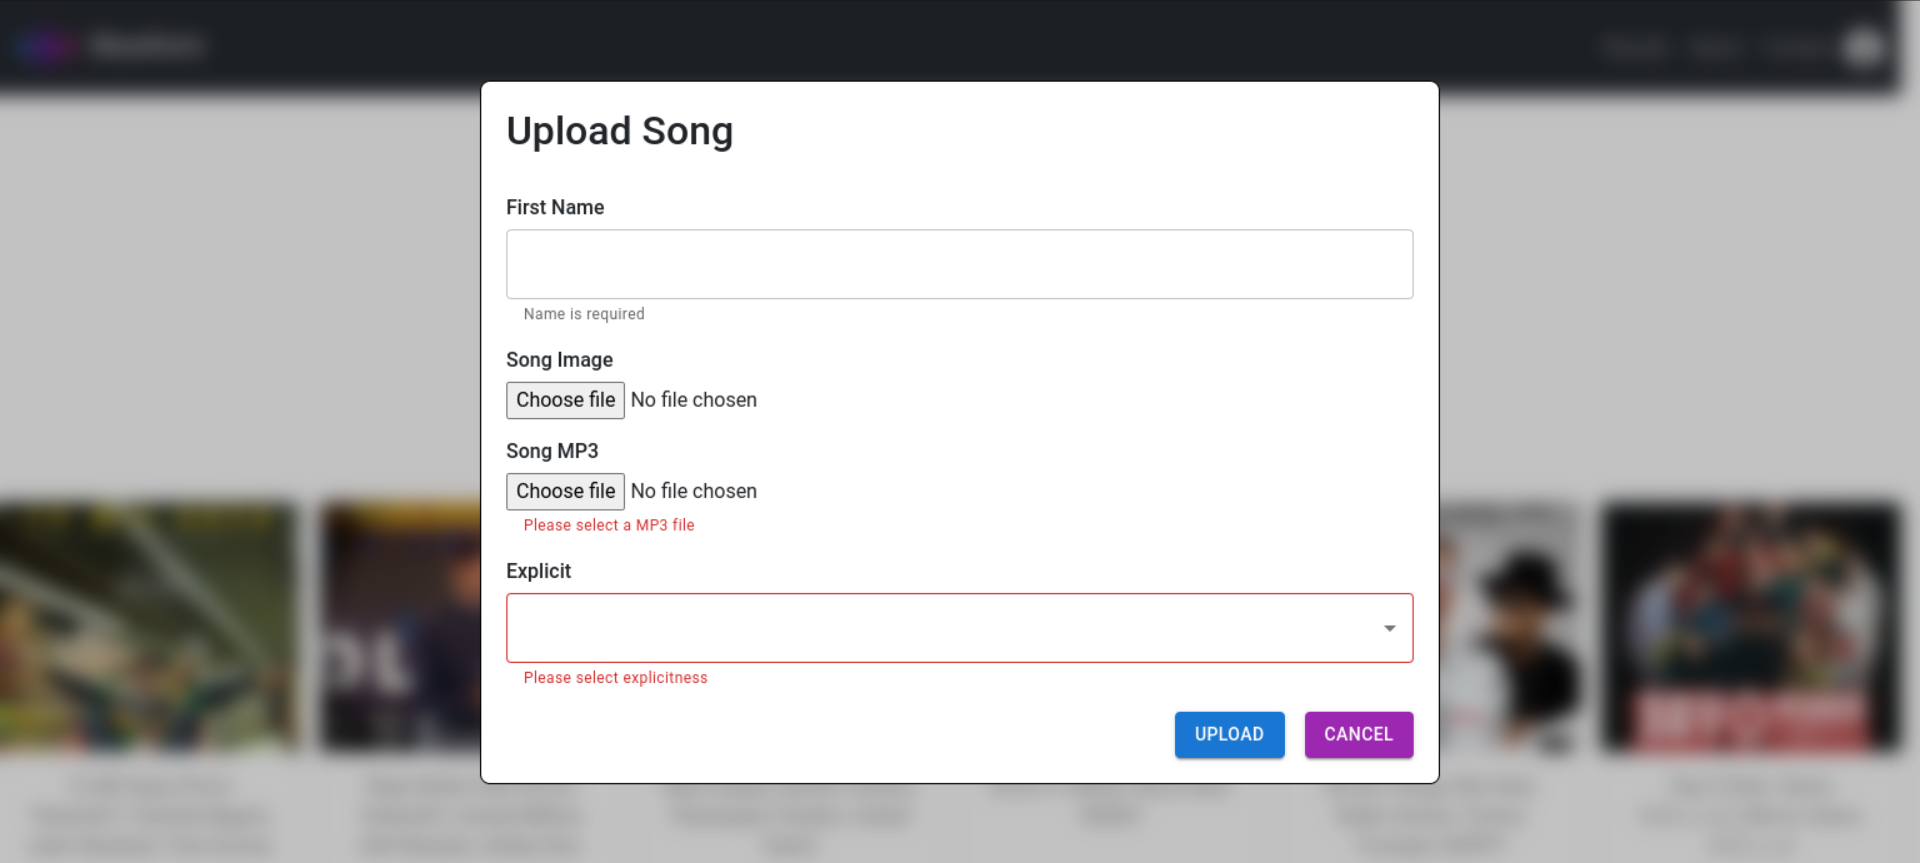
\includegraphics[height=.4\linewidth]{screenshots/8.upload.png}
    \caption{Upload Page}
   
\end{figure}

\begin{figure}[h]
    \centering
    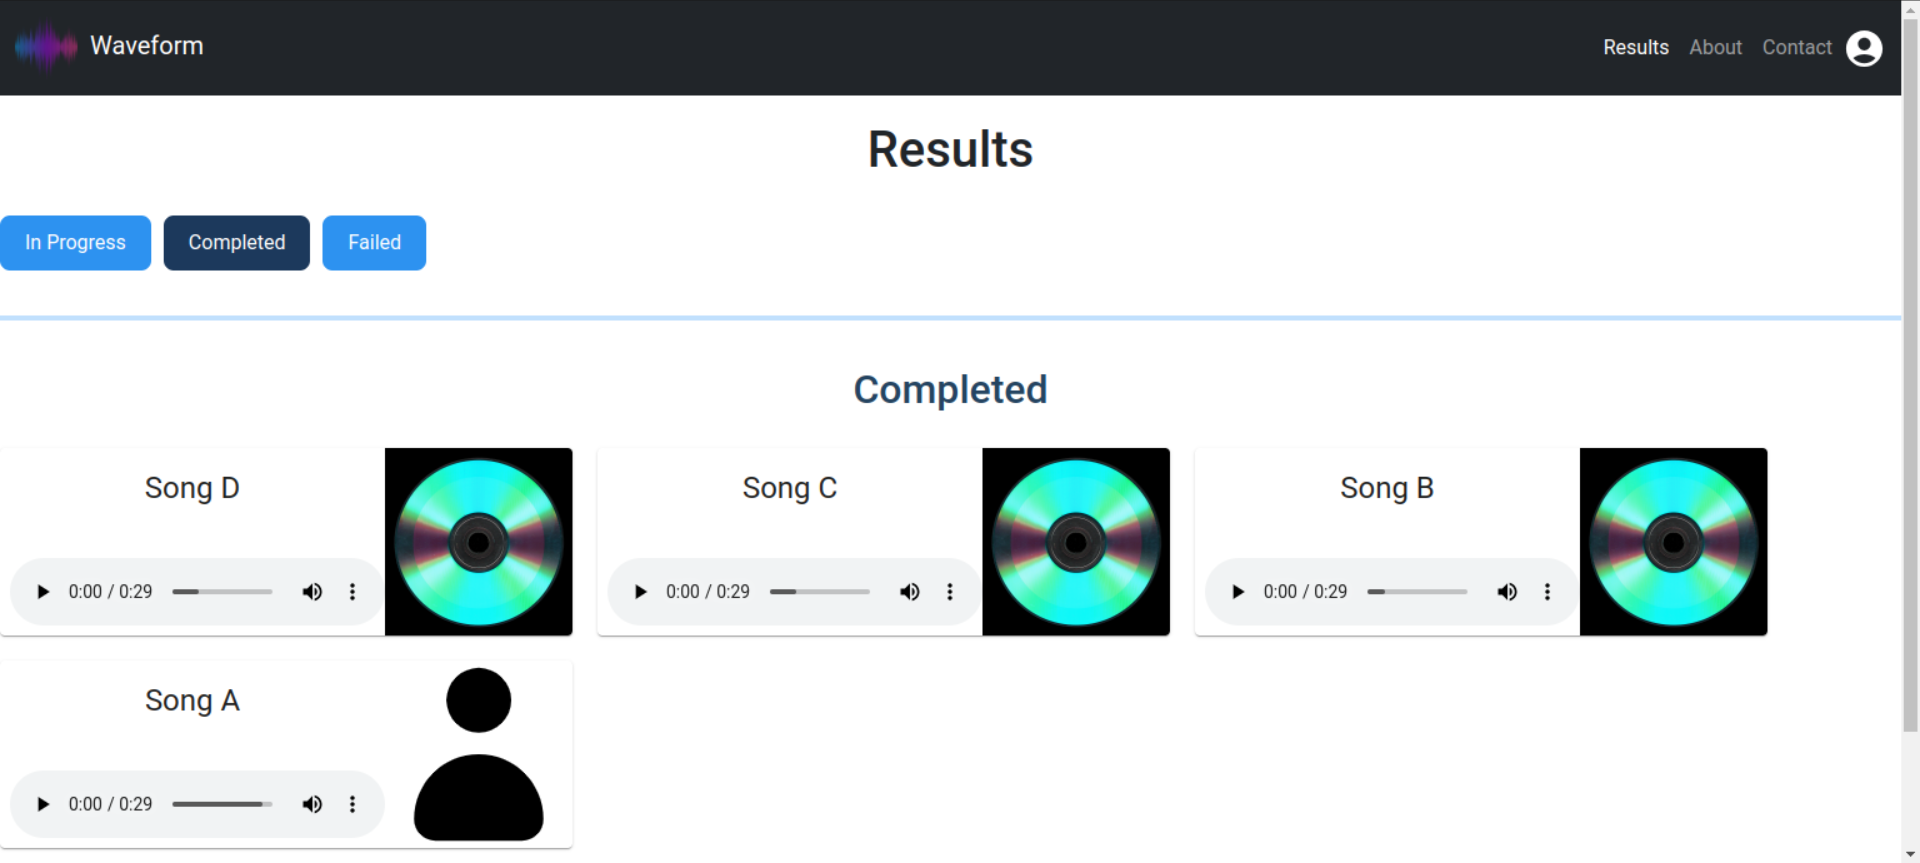
\includegraphics[height=.5\linewidth]{screenshots/9.results.png}
    \caption{Results Page}
 
\end{figure}

\begin{figure}[h]
    \centering
    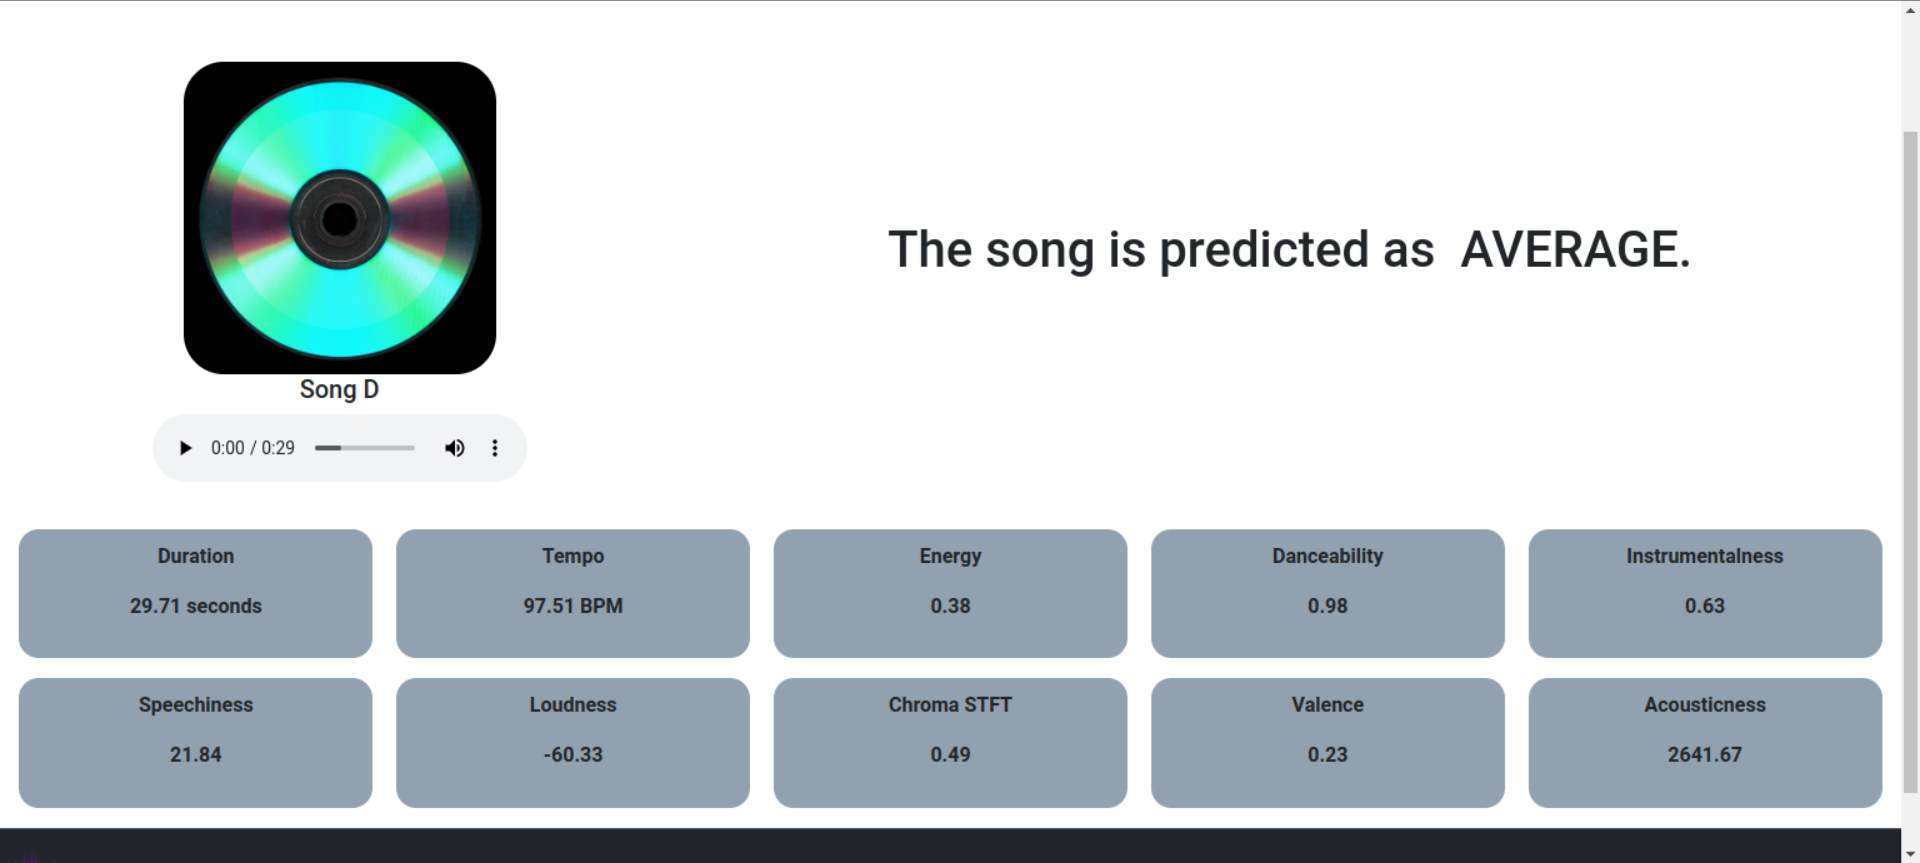
\includegraphics[height=.5\linewidth]{screenshots/10.stat-result.png}
    \caption{Stat-Result Page}
 
\end{figure}

\begin{figure}[h]
    \centering
    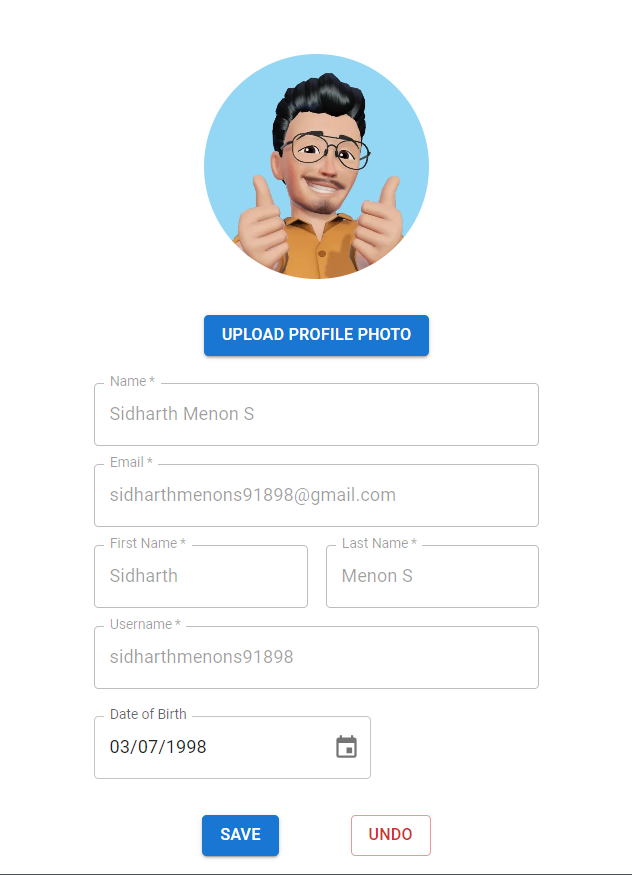
\includegraphics[width=.33\linewidth]{screenshots/12.profile.png}
    \caption{Profile Page}
    
\end{figure}

\begin{figure}[h]
    \centering
    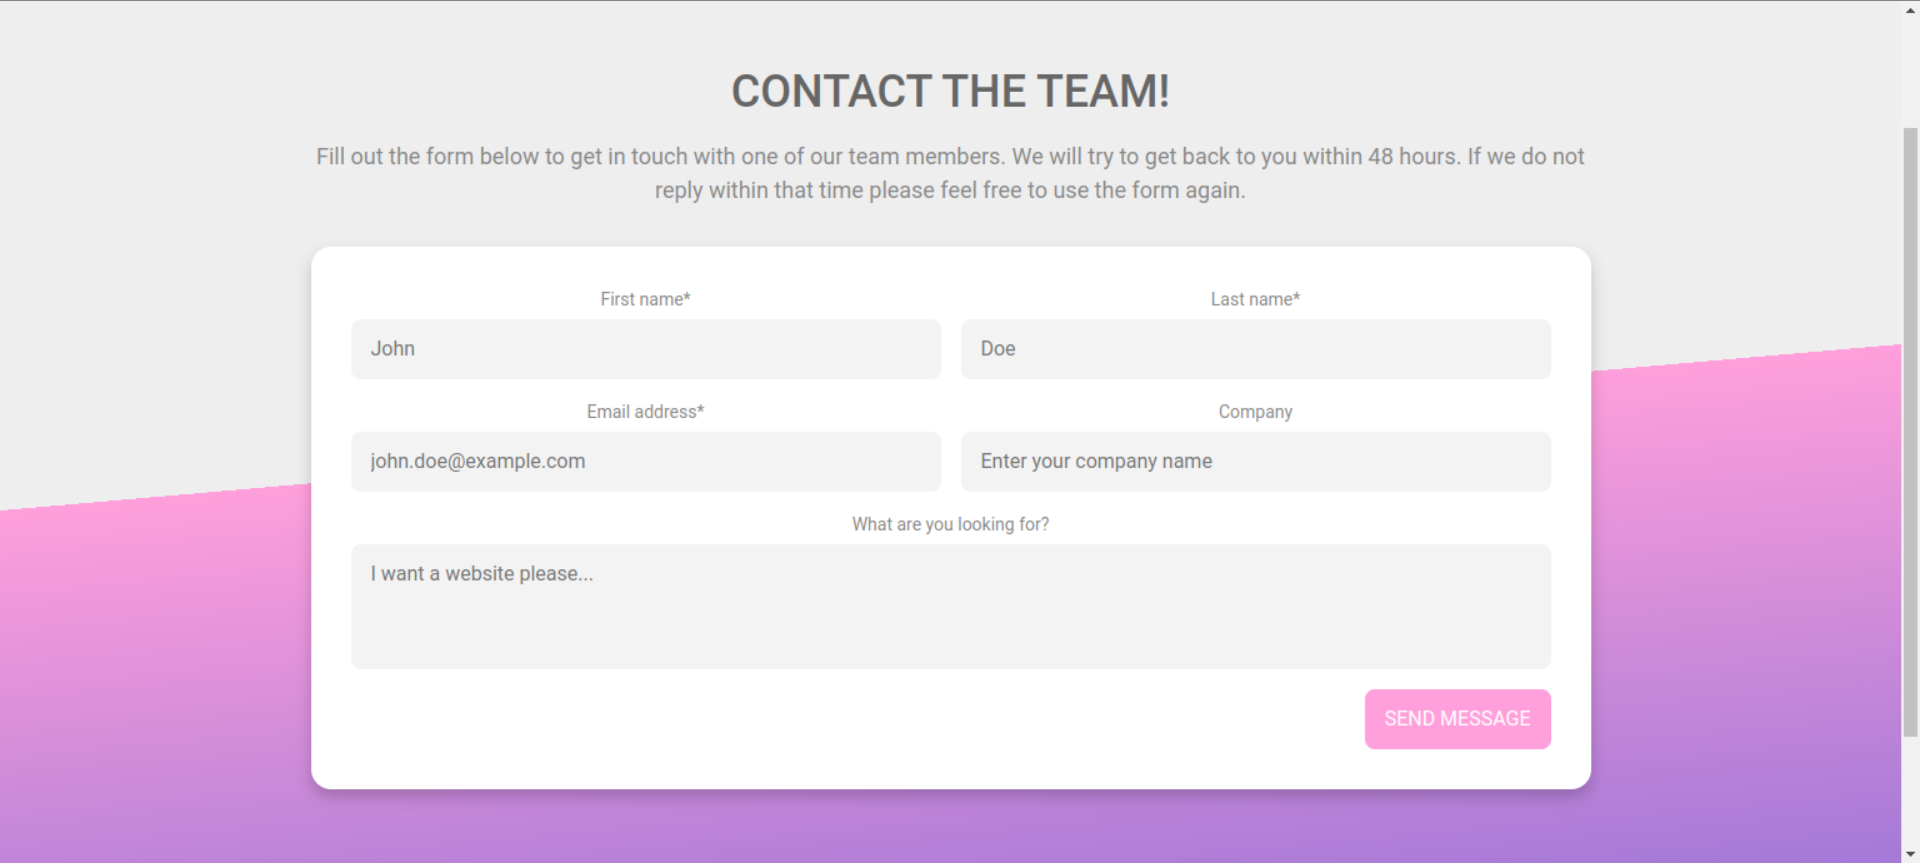
\includegraphics[height=.45\linewidth]{screenshots/11.contact.png}
    \caption{Contact Page}
\end{figure}
\begin{figure}[h]
    \centering
    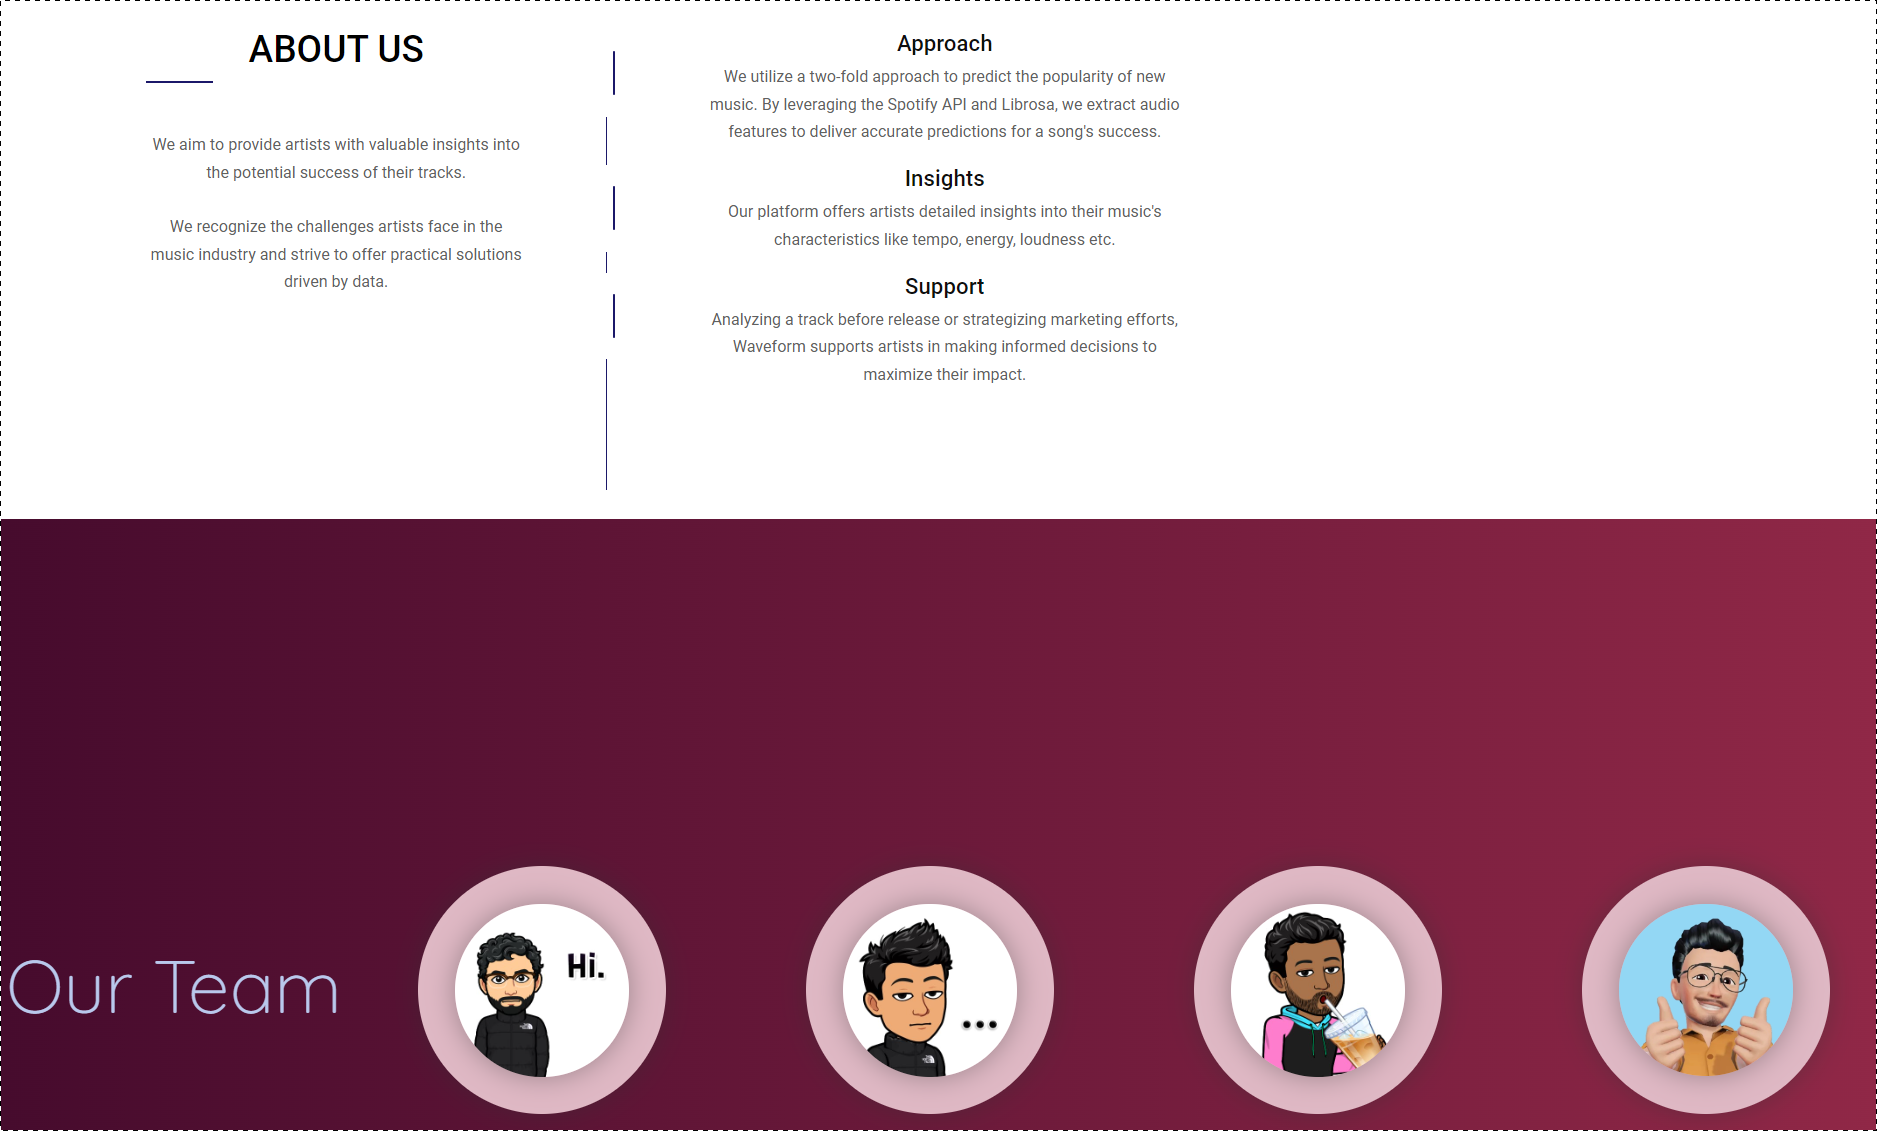
\includegraphics[height=.6\linewidth]{screenshots/about.png}
    \caption{About Page}
\end{figure}
    
% \chapter{Results}
% % \clearpage
%  \section{Output}
%  \begin{figure}[h]
%     \centering
%     \includegraphics[width=1\linewidth]{images/high-level-1.png}
%     \caption{High Level Result}
   
% \end{figure}

% \begin{figure}[h]
%     \centering
%     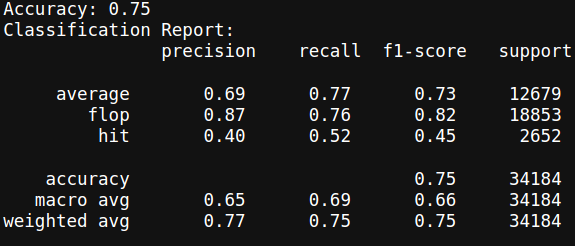
\includegraphics[width=1\linewidth]{alby.png}
%     \caption{Low Level Result}
   
% \end{figure}
% \clearpage

\chapter{Results}

\section{High Level Model}

The high level model results demonstrate significant results. During the randomized cross-validation process, Adaboost achieved an accuracy of 75\%, Random Forest achieved 80\%, and XGBoost reached 80\%. Among these, XGBoost outperformed the others and was selected as the best model after grid search optimization, achieving an accuracy of 81\%.

\begin{figure}[H]
    \centering
    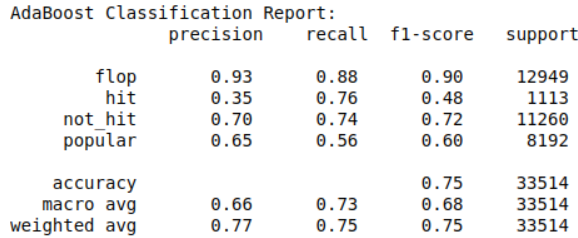
\includegraphics[width=0.8\linewidth]{results/highlevel_ada_random.png}
    \caption{Randomized CV: Adaboost}
\end{figure}

\begin{figure}[H]
    \centering
    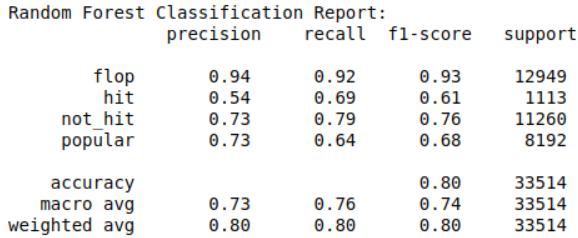
\includegraphics[width=0.8\linewidth]{results/highlevel_rf_random.png}
    \caption{Randomized CV: Random Forest}
\end{figure}

\begin{figure}[H]
    \centering
    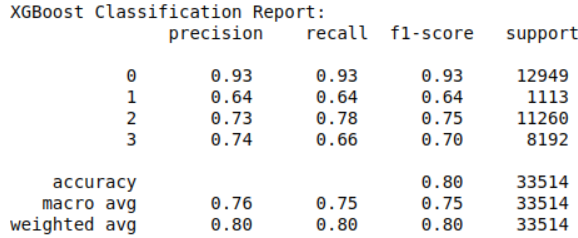
\includegraphics[width=0.8\linewidth]{results/highlevel_xgb_random.png}
    \caption{Randomized CV: XGBoost}
\end{figure}

\begin{figure}[H]
    \centering
    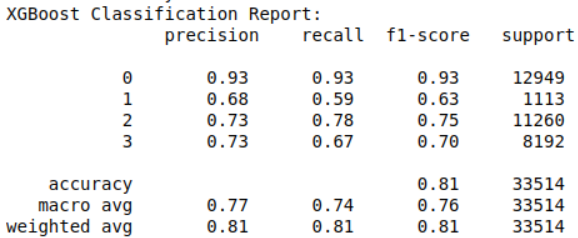
\includegraphics[width=0.8\linewidth]{results/highlevel_xgb_grid.png}
    \caption{Grid Search: XGBoost}
\end{figure}

\section{Low Level Model}

The low level model results also show promising outcomes. Adaboost attained an accuracy of 56\% during randomized cross-validation, Random Forest achieved 58\%, and XGBoost reached 58\%. However, after grid search optimization, XGBoost emerged as the best model with an accuracy of 59\%.

\begin{figure}[H]
    \centering
    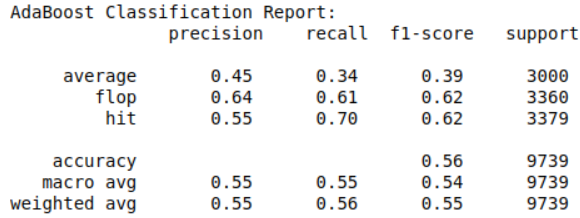
\includegraphics[width=0.8\linewidth]{results/lowlevel_ada_random.png}
    \caption{Randomized CV: Adaboost}
\end{figure}

\begin{figure}[H]
    \centering
    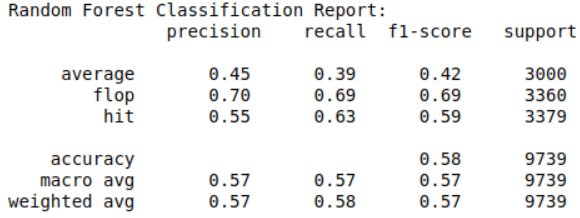
\includegraphics[width=0.8\linewidth]{results/lowlevel_rf_random.png}
    \caption{Randomized CV: Random Forest}
\end{figure}

\begin{figure}[H]
    \centering
    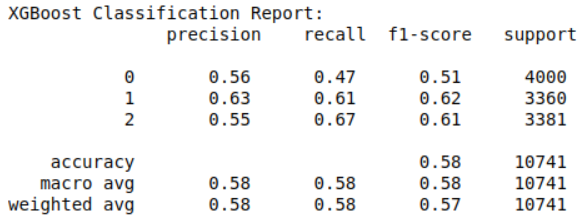
\includegraphics[width=0.8\linewidth]{results/lowlevel_xgb_random.png}
    \caption{Randomized CV: XGBoost}
\end{figure}

\begin{figure}[H]
    \centering
    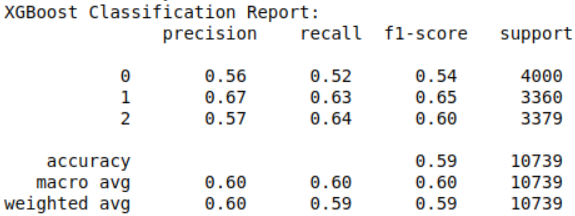
\includegraphics[width=0.8\linewidth]{results/lowlevel_xgb_grid.png}
    \caption{Grid Search: XGBoost}
\end{figure}

\clearpage

\chapter{Conclusion}

In this project, we presented Waveform,as a web application aimed at predicting the popularity of  music on Spotify as well as songs uploaded by users. By leveraging advanced machine learning techniques and audio analysis tools, Waveform addresses the longstanding challenge faced by musicians in assessing the potential success of their tracks, even though individual preferences may vary.
\\\\
Through the integration of high-level and low-level feature extraction methods, Waveform provides a comprehensive approach to understanding the dynamics of music popularity. The utilization of the Spotify API for high-level feature extraction and librosa for low-level feature extraction allows for a better analysis of audio features, providing valuable insights into the characteristics of songs.Our experiments with machine learning models, including Random Forest, AdaBoost, and XGBoost classifiers, demonstrate the effectiveness of ensemble learning approaches in predicting song popularity. These models, trained on a diverse range of audio features, showcase the importance of feature engineering and selection in improving prediction accuracy.
\\\\
Furthermore, Waveform offers a user-friendly interface that empowers musicians and music enthusiasts to explore and interpret audio features, enabling informed decision-making in music production and release strategies. In conclusion, Waveform is a tool that can help you  predict song popularity and analyze audio features. 

\chapter{Future Scope}

\begin{itemize}
\item \textbf{Advanced ML Techniques:} Explore the integration of advanced machine learning techniques such as neural networks and deep learning models to enhance the accuracy and sophistication of popularity prediction algorithms. These techniques have the potential to uncover complex patterns and relationships within music data that traditional models may overlook.

\item \textbf{NLP Integration for Lyrics Analysis:} Incorporate natural language processing (NLP) techniques by scraping lyrics data from sources like Genius or Musixmatch. By converting text into numerical features, NLP models can be applied to analyze lyrical content and its impact on music popularity, providing a more comprehensive understanding of song characteristics.

\item \textbf{Data Expansion:} Address constraints in data availability by collecting more diverse and extensive datasets. This expansion may be limited in the current version due to storage, computation, and time constraints. With access to larger datasets, models can be trained on a wider range of music genres, demographics, and cultural contexts, improving the robustness and generalization of predictions.

\item \textbf{Continuous Model Improvement:} Establish mechanisms for continuous model improvement through ongoing monitoring, evaluation, and adaptation to evolving music trends and user preferences. This iterative approach ensures that the prediction models remain up-to-date and relevant in a dynamic music landscape.

\end{itemize}

\clearpage

   
% \begin{thebibliography}{999}
% \addcontentsline{toc}{chapter}{References}
% \bibitem{}


% \end{thebibliography}

\addcontentsline{toc}{chapter}{References}
\bibliographystyle{IEEEtran} % We choose the "plain" reference style
\bibliography{References}

\end{document}
